\documentclass[12pt,a4paper,final]{report}
\usepackage[english]{babel}
\usepackage[fleqn]{amsmath}
\usepackage{amsfonts}
\usepackage{amssymb}
\usepackage{mathptmx}
\usepackage{fancyhdr}
\usepackage{graphicx}
\usepackage{array}
\usepackage{enumitem}
\usepackage{booktabs}

\usepackage[%
    a4paper,
%   includeheadfoot,
    head=0.762cm,  % distance from bottom of header to block of text aka \headsep e.g. \baselineskip
    foot=0.762cm,  % distance from top of footer to block of text aka \footskip
    headheight=12pt,     % height for the header block (no equivalent for footer)
%   heightrounded,       % ensure an integer number of lines
    marginparwidth=2cm,  % right marginal note width
    marginparsep=2mm,    % distance from text block to marginal note box
%   height=\textheight,  % height of the text block
%   width=\textwidth,    % width of the text block
    top=1.7cm,           % distance of the text block from the top of the page
    bottom=1.4cm,
    left=1.9cm,
    right=1.9cm,
%    showframe,           % show the main blocks
%    verbose,             % show the values of the parameters in the log file
]{geometry}

\pagestyle{fancy}
\fancyhf{}

\lhead{\bfseries Avoiding Road Traffic Congestion using Dynamic Traffic Assignment Approach}
\cfoot{DEPARTMENT OF COMPUTER ENGINEERING, PESMCOE PUNE}
\rfoot{\bfseries \thepage}

\usepackage[table]{xcolor}
\newcolumntype{P}[1]{>{\centering\arraybackslash}p{#1}}
\newcolumntype{M}[1]{>{\centering\arraybackslash}m{#1}}

\renewcommand{\footrulewidth}{0.4pt}

\title{Title}
\graphicspath{ {Images/} }

\usepackage{tikz}
\usetikzlibrary{calc}
\usepackage{eso-pic}

\usepackage{titlesec}
\titleformat{\section}[block]
  {\fontsize{16}{18}\bfseries}
  {\thesection}
  {1em}
  {}
\titleformat{\subsection}[block]
  {\fontsize{14}{15}\bfseries}
  {\thesubsection}
  {1em}
  {}

\usepackage{blindtext}
\usepackage{tocloft}
\renewcommand{\cfttoctitlefont}{\hspace*{\fill}\Huge\bfseries}
\renewcommand{\cftaftertoctitle}{\hspace*{\fill}}
\renewcommand{\cftlottitlefont}{\hspace*{\fill}\Huge\bfseries}
\renewcommand{\cftafterlottitle}{\hspace*{\fill}}
\renewcommand{\cftloftitlefont}{\hspace*{\fill}\Huge\bfseries}
\renewcommand{\cftafterloftitle}{\hspace*{\fill}}

\newcommand{\abbrlabel}[1]{\makebox[6cm][l]{\textbf{#1}\ \dotfill}}
\newenvironment{abbreviations}{\begin{list}{}{\renewcommand{\makelabel}{\abbrlabel}}}{\end{list}}

\DeclareRobustCommand{\gobblefive}[5]{}
\newcommand*{\SkipTocEntry}{\addtocontents{toc}{\gobblefive}}

\usepackage{hyperref}
\hypersetup{
    colorlinks=true,
    linkcolor=black,
    citecolor=black,
}

\begin{document}
\begin{center}
\thispagestyle{empty}
\vspace*{1cm}
A PARTIAL PROJECT REPORT
\vspace*{0.75cm}

ON
\vspace*{0.75cm}

\Large
Avoiding Road Traffic Congestion using Dynamic Traffic Assignment Approach
\vspace*{0.75cm}


\vspace*{0.5cm}
SUBMITTED BY
\vspace*{0.35cm}
\linebreak
Adil Hussain : B120314204
\linebreak
Mohammad Moheed Inamdar : B120314249
\linebreak
Ajay Singh Rajpurohit : B120314310
\linebreak
Utkarsh Alone : B120314207
\linebreak

\vspace*{0.5cm}
UNDER THE GUIDENCE OF
\vspace*{0.35cm}
\linebreak
Mrs. Deepti Nirwal
\vspace*{0.3cm}
\normalsize
\begin{figure}[h]
\begin{center}

\includegraphics[width=3.5cm, height=4.0cm]{logo.png}
\end{center}
\end{figure}



\large
\vspace*{0.3cm}
DEPARTMENT OF COMPUTER ENGINEERING
\linebreak
P.E.S MODERN COLLEGE OF ENGINEERING
\linebreak
PUNE - 411005.
\linebreak
$[$2017 - 18$]$ 
\end{center}
\newpage


\thispagestyle{empty}
\vspace*{1.3cm}
\begin{center}

\includegraphics[width=3.5cm, height=4.0cm]{logo.png}
\end{center}
\begin{center}
\Large
Progressive Education Society's \\
\textbf{Modern College of Engineering} \\
Department of Computer Engineering\\
Shivajinagar, Pune - 411005. \\
\vspace{1cm}

\underline{\textbf{CERTIFICATE}}
\end{center}
\normalsize
\vspace{0.5cm}
This is to certify that the following students of Final Year Computer Engineering have successfully completed the preliminary analysis and design of project entitled ``\emph{Avoiding Road Traffic Congestion using Dynamic Traffic Assignment Approach}'' for the organization ``PES Modern College Of Engineering'' \\
The Group Members names are: \hspace{0.1cm} Adil Hussain \\
\hspace*{5.7cm} Mohammad Moheed Inamdar \\
\hspace*{5.7cm} Ajay Singh Rajpurohit \\
\hspace*{5.7cm} Utkarsh Alone. \vspace{0.5cm}\\
This is in partial fulfilment of Bachelor of Computer Engineering under Savitribai Phule Pune University. \vspace{1cm}\\
Date: \vspace{1cm} \\
(Mrs. Deepti Nirwal)
\hspace*{2.5cm}(Prof. Dr. Mrs. S. A. Itkar) \\
\hspace*{0.5cm}Internal Guide 	 
\hspace{4.5cm}Head
\hspace{5.5cm}External Examiner \\
\hspace*{4.5cm}Department of Computer Engineering \\


\thispagestyle{empty}
\Large
\begin{center}
\chapter*{\centering Acknowledgement}
\end{center}
\normalsize
It gives us pleasure in presenting the partial project report on \textbf{`Avoiding Road Traffic Congestion using Dynamic Traffic Assignment Approach'}.\\

Firstly, we would like to express our indebted appreciation to our internal guide \textbf{Mrs. Deepti Nirwal}. Her constant guidance and advice played very important role in making the execution of the report. She always gave us her suggestions, that were crucial in making this report as flawless as possible.\\

We would like to express our gratitude towards \textbf{Prof. Dr. Mrs. S. A. Itkar} Head of Computer Engineering Department, PES Modern College of Engineering for her kind co-operation and encouragement which helped us during the completion of this report.\\

Also we wish to thank our Principal, \textbf{Prof. Dr. Mrs. K. R. Joshi} and all faculty members for their whole hearted co-operation for completion of this report. We also thank our laboratory assistants for their valuable help in laboratory. \\

Last but not the least, the backbone of our success and confidence lies solely on blessings of dear parents and lovely friends.

\begin{flushright}
Adil Hussain\\
Mohammad Moheed Inamdar\\
Ajay Singh Rajpurohit\\
Utkarsh Alone\\
\end{flushright}


\pagestyle{plain} 
\cleardoublepage
\pagenumbering{gobble}
\tableofcontents
\newpage

\pagenumbering{roman}
\Large
\chapter*{\centering Abstract}
\addcontentsline{toc}{chapter}{Abstract}
\normalsize
\noindent

Traffic management is a tedious task riddled with a lot of uncertainity of buildup and flow changes. The largest issue regarding Traffic Management is its unpredictability of changes. This Project aims to tackle this issue with the use of incremental changes that counteract signs of Traffic buildup. The idea is to detect changes in the traffic density (from cycle to cycle) and slowly increase/decrease signal timings for the growing/shrinking route density or overall. \\
This allows us to do 2 things at once, viz. 
	\begin{enumerate}
		\item Prepare and provide proportional timings to each road of the signal and 
		\item Dynamically increase/decrease the overall signal cycle time based on density growth/reduction.
	\end{enumerate}	 
 Our system is ideal for use in a Smart City environment or any environment that provides GSM internet or mobile data abilities near the roads. 
\newpage

\listoffigures
\addcontentsline{toc}{chapter}{List of Figures}
\newpage
\listoftables
\addcontentsline{toc}{chapter}{List of Tables}
\newpage

\chapter*{\centering List of Abbreviations}
\begin{abbreviations}
\item[API] Application Programming Interface
\item[GTAPI] Google Traffic API
\item[JSON] JavaScript Object Notation
\item[XML] eXtensible Markup Language
\item[CSS] Cascading Style Sheets
\item[VANET] Vehicular Ad-hoc NETwork
\item[IoT] Internet of Things
\item[WSN] Wireless Sensor Network
\item[IDE] Integrated Development Environment
\item[GSM] Global Systems for Mobile
\item[MOTUS] Microscopic Open Traffic Simulator : http://homepage.tudelft.nl/05a3n/
\item[UI] User Interface
\item[P2P] Peer to Peer
\item[NIC] Network Interface Card

\end{abbreviations}

\addcontentsline{toc}{chapter}{List of Abbreviations}
\newpage
\pagestyle{fancy}
 
\newcommand{\hsp}{\hspace{0pt}}
\titleformat{\chapter}[hang]
{\flushright\fontseries{b}\fontsize{80}{100}\selectfont}{\fontseries{b}\fontsize{72}{84}\selectfont\textcolor{black}\thechapter\hsp}{0pt}
{.\\ \Huge\bfseries}
[]\titlespacing*{\chapter}{0pt}{540pt}{20pt}	

%\pagenumbering{gobble}
\pagenumbering{arabic}

\AddToShipoutPictureBG*{%
\begin{tikzpicture}[overlay,remember picture]
\draw[line width=1.5pt]
    ($ (current page.north west) + (0.7cm,-0.7cm) $)
    rectangle
    ($ (current page.south east) + (-0.7cm,0.7cm) $);
\draw[line width=1.5pt]
    ($ (current page.north west) + (0.9cm,-0.9cm) $)
    rectangle
    ($ (current page.south east) + (-0.9cm,0.9cm) $);
\end{tikzpicture}
}
\chapter{Introduction}
\thispagestyle{empty}
\newpage

\section{Brief Description}

The problem statement describes a problem that is very complex to deal with. It contains many variables like density of traffic, frequency of input, probability of failure, location of failure, area/capacity of channel, etc. Finding an equation that defines the flow in the network using these variables is a tedious task as the behaviour of such networks is not defined with respect to each variable. Also, conducting experiments over the network in an attempt to define relations between one variable and the traffic (keeping all other variables constant) is limited to simulations. Such experiments cannot be conducted in the real world.\\

Many solutions use IoT devices embedded inside vehicles (or VANET) that solve this problem by finding the density and urgency of each vehicle to adjust traffic signal timings. Other solutions use WSN to identify traffic density using infrared lasers across the road to mark low, medium and high traffic. This technique adapts the traffic signal based on the amount of backlog in each lane that builds up over the "red" duration of the traffic signal for a given lane.\\

We observe that these variables have slow variations over time for the case of Road Traffic. This allows us to observe activities as they happen and make changes to accomodate the traffic. Our solution uses Incremental Approach since it is a common approach used to tackle problems in slowly changing systems. It solves these issues by developing a continual monitor-evaluate-modify loop that tends to adapt to problems with no single solution. 

\section{Problem Statement}
Devise a Distributed Control system to solve the Traffic Assignment Problem on City Roads.

\section{Objectives of the Project}
\begin{enumerate}
\item
To Observe Current Traffic Conditions.

\item
To Mediate Road Traffic Flow.

\item
To Dynamically Control Traffic Signals.

\end{enumerate}

\section{Scope of the Project}
\begin{enumerate}
\item
IoT Based Traffic Signal Control (Arduino)
\item
Decentralized Algorithm to create changes in Signal timings
\end{enumerate}

\newpage

\AddToShipoutPictureBG*{%that bordered page
\begin{tikzpicture}[overlay,remember picture]
\draw[line width=1.5pt]
    ($ (current page.north west) + (0.7cm,-0.7cm) $)
    rectangle
    ($ (current page.south east) + (-0.7cm,0.7cm) $);
\draw[line width=1.5pt]
    ($ (current page.north west) + (0.9cm,-0.9cm) $)
    rectangle
    ($ (current page.south east) + (-0.9cm,0.9cm) $);
\end{tikzpicture}
}

\chapter{Literature Survey}
\thispagestyle{empty}
\newpage
\newcolumntype{P}[1]{>{\centering\arraybackslash}p{#1}}
\section{Literature Survey}
\begin{table}[!ht]
\centering
\begin{tabular}{ P{1cm} P{2.7cm} P{1.8cm} P{2.4cm} P{2.4cm}}

Sr. No. & Title & Author & Journal & Purpose \\
\hline
& & & & \\
1 & An Integrated and Scalable Platform for Proactive Event-Driven Traffic Management 
& Alain Kibangou, Alexander Artikis \textit{et. al}
& ArXiv.org, March 2017
& SPEEDD project, ML predictive approach \\

& & & & \\

2 & Self-organizing Traffic Lights & Carlos Gershenson & Complex Systems, 2005
& Naive Distributed Traffic Signal Control \\

& & & & \\

3 & Centralized and Localized Data Congestion Control Strategy for Vehicular Ad Hoc Networks Using a Machine Learning Clustering Algorithm
& Nasrin Taherkhani and Samuel Pierre
& IEEE Transactions on Intelligent Transportation Systems, 2016
& Example of Ad-Hoc Approach (VANET) \\
& & & & \\
\hline
\end{tabular}
\caption{Literature Survey}
\end{table}
\newpage



\AddToShipoutPictureBG*{
\begin{tikzpicture}[overlay,remember picture]
\draw[line width=1.5pt]
    ($ (current page.north west) + (0.7cm,-0.7cm) $)
    rectangle
    ($ (current page.south east) + (-0.7cm,0.7cm) $);
\draw[line width=1.5pt]
    ($ (current page.north west) + (0.9cm,-0.9cm) $)
    rectangle
    ($ (current page.south east) + (-0.9cm,0.9cm) $);
\end{tikzpicture}
}
\chapter{Design Details}
\thispagestyle{empty}
\newpage
\section{Requirements Analysis}
\subsection{Project Requirements:}
		The Software Requirements are:
	\begin{itemize}
		\item Arduino IDE
		\item Redis Database - JSON/XML
		\item GTAPI
		\item Apache Tomcat
		\item Sublime editor
		\item Python v3.5
		\item JavaScript - Vue.JS, JQuery
		\item CSS - Sass
	\end{itemize}
\vspace*{10pt}
		The Hardware Requirements are:
	\begin{itemize}
		\item Arduino Uno Rev3
		\item 3G/4G GSM Shield
	\end{itemize}
\vspace*{10pt}
		The System Requirements are:
	\begin{itemize}
		\item Windows/Linux Operating System
		\item MOTUS
		\item Python's matplotlib.
	\end{itemize}

\newpage 

\subsection{Problem Description:}
	The Issues in Indian Traditional Traffic Management systems are that they are:
	\begin{enumerate}
		\item \underline{Inflexible:} They do not adapt to changing situations in real time. In case of \emph{accidents} or \emph{disputes}, the traffic piles up rather quickly into a 1-3 hour jam.
		\item \underline{Inadaptive:} Traditional approach do not optimize signal's waiting times for each line according to the traffic in the incoming lanes.
		\item \underline{Uncoordinated:} Situations that arise in one area usually produce effects on nearby regions, though the remedial measures do not reach these other areas quickly enough.
		\item \underline{Manual or Preset Control:} The timings of each signal and the ability to switch them on/off need human interaction which are slow and/or inefficient.
	\end{enumerate}

\subsection{Solution Description:}
	We propose a solution to these problem by first making some assumptions:
	\begin{itemize}
		\item The roads do not vary in width by a huge factor near the signal (500m).
		\item People do not usually jump the signal.
		\item Most travellers carry their smartphones.
	\end{itemize}
		
	Our solution to the problem uses a Mathematical system that is similar to one which is built to balance weights.\\
		
	Let's assume that on a signal, the densities of incoming traffic is $D_{N}, D_{E}, D_{W}$ and $D_{S}$ (may vary as per number of directions/lanes).
	We then use the summation of these densities to decide upon the cycle time (C).\\
\begin{equation}
	C = \frac{\sum D_{d}}{C_{avg}}
\end{equation}

			where $C_{avg}$ is the average Cycle time among it's neighbours.
	Using these we divide the cycle time C into 4 parts (as per number of directions/lanes). These 4 cycle parts are used as total alloted time per lane.\\
		
	From this alloted time or slots, we first identify which are too low or too high. These are categorized as $Min\_C$ and $Max\_C$ respectively. This is to ensure there is some meaningful minimal and some bounding maximum cycle slots to consider. Note that though there is a single $Min\_C$, there are multiple $Max\_C$ for allowing a one way routed traffic on a cross section (Work Day traffic flows are usually one directional).\\
		
	Then we split the slot time into Red, Green and Yellow timings of the Signal. These values are then provided to the Signal for control.
		
	The higher orders of $Max\_C$ (also known as $Max\_C_{i}$) come with a correctional cost. This cost is added back to the Cycle slot in the following manner.\\
	\begin{equation}
			C_{corrected} = C + \sum_{i = 1}^{i = n} Cost(i)
	\end{equation}
			
\newpage
	The tendency of this correctional cost is to release more traffic in order to reduce the incoming traffic. This causes the densities to appear dynamic. The net result of this operation over time is to increase the traffic fluidity while economizing the whole cycle time. When these densities approach each other, the higher orders of $Max\_C$ are reduced to either $Max\_C$ or lower cycle slot time. This tends to make original cycle slot to the corrected cycle time.\\
			
	Hence this Mathematical system automatically balances itself which in turn smoothen out traffic. Consequently, this system works independent of it's own instances and hence is a purely decentralized system.

\subsection{Project Outcome:}
	On completion, we will have desgined:
	\begin{itemize}
		\item User's Software perspective:	
		\begin{enumerate}
			\item A Signal Controller software.
			\item A web interface to see signal timings generated by the system.
			\item A web interface to check locations of jams and/or other bottlenecks.
			\item A web interface to change/modify the routes (actual signals and associated lanes are shut down or rerouted) on-the-fly.
		\end{enumerate}
		
		\item User's Hardware perspective:
		\begin{enumerate}
			\item A Signal Controller board.
		\end{enumerate}
	\end{itemize}
\section{SRS}

\subsection{Necessary Functions:}
\begin{itemize}
	\item Dynamically scale signal timings as per lane's incoming traffic.
	\item Dynamically reduce/eliminate the onset of traffic jams.
	\item On-the-fly Route configuration and modification.
	\item Visible Timings (Exposed info) of each signal controller.
	\item Authentication and User creation for Traffic Control Administrator(s).
	\item Automatic Detection, Reporting and Adaptation to Signal Controller Failures.
\end{itemize}

\subsection{Desirable Functions:}
\begin{itemize}
	\item Android application to warn users of new changes in the Traffic system.
	\item Android webview of web interface to see Traffic status.
	\item Provision for adapting to emergency services (ambulance,fire brigade, etc.)
\end{itemize}

\subsection{Interface Requirements:}
\underline{User interfaces:}
\begin{enumerate}
	\item UI for visitors to see signal timings.
	\item UI for authentication of Traffic Control Administrators.
	\item UI for editing (with support for undo/redo) routes and signal operation.
	\item Exposed API for using non-authenticated functionalities outside of UI.
\end{enumerate}

\underline{Hardware Interfaces}
\begin{enumerate}
	\item A hidden P2P communication strategy for real-time monitoring network status.
	\item Automatic route expansion in case of signal controller failure.
\end{enumerate}
\underline{Software Interfaces:}
\begin{enumerate}
	\item Hidden P2P localhost server for notifying lane neighbours.
	\item Web server to Controller interface for operating on controller (switching on/off, changing route, watching timings).
\end{enumerate}

\underline{Communication Interfaces:}
\begin{enumerate}
	\item 3G/4G GSM internet connection.
	\item IoT connectivity between signal controllers.
\end{enumerate}

\subsection{System Features:}
	\begin{enumerate}
		\item \underline{Speed} - Use of Microcontroller makes sure that the hardware doesn't prove to be the bottleneck of the System's operation.
		\item \underline{Consistency} - Use of Microcontrollers allow the software to not generate corrupt structures as the code will not change or get corrupted from use (as is the case of overheated microprocessor systems).
		\item \underline{Decentralized} - No single point of failure exists in this system.
		\item \underline{Adapative} - System is capable of handling many situations by itself in real time.
		\item \underline{Security} - Inner working of Authentication and Modifications uses Hashes that are untraceable to their sources. Hence they mark events instead of Credentials or System's Data.
	\end{enumerate}
\newpage

\section{Design Phase :}
\subsection{Architecture Block Diagram}
	\begin{figure}[!h]
		\begin{center}
			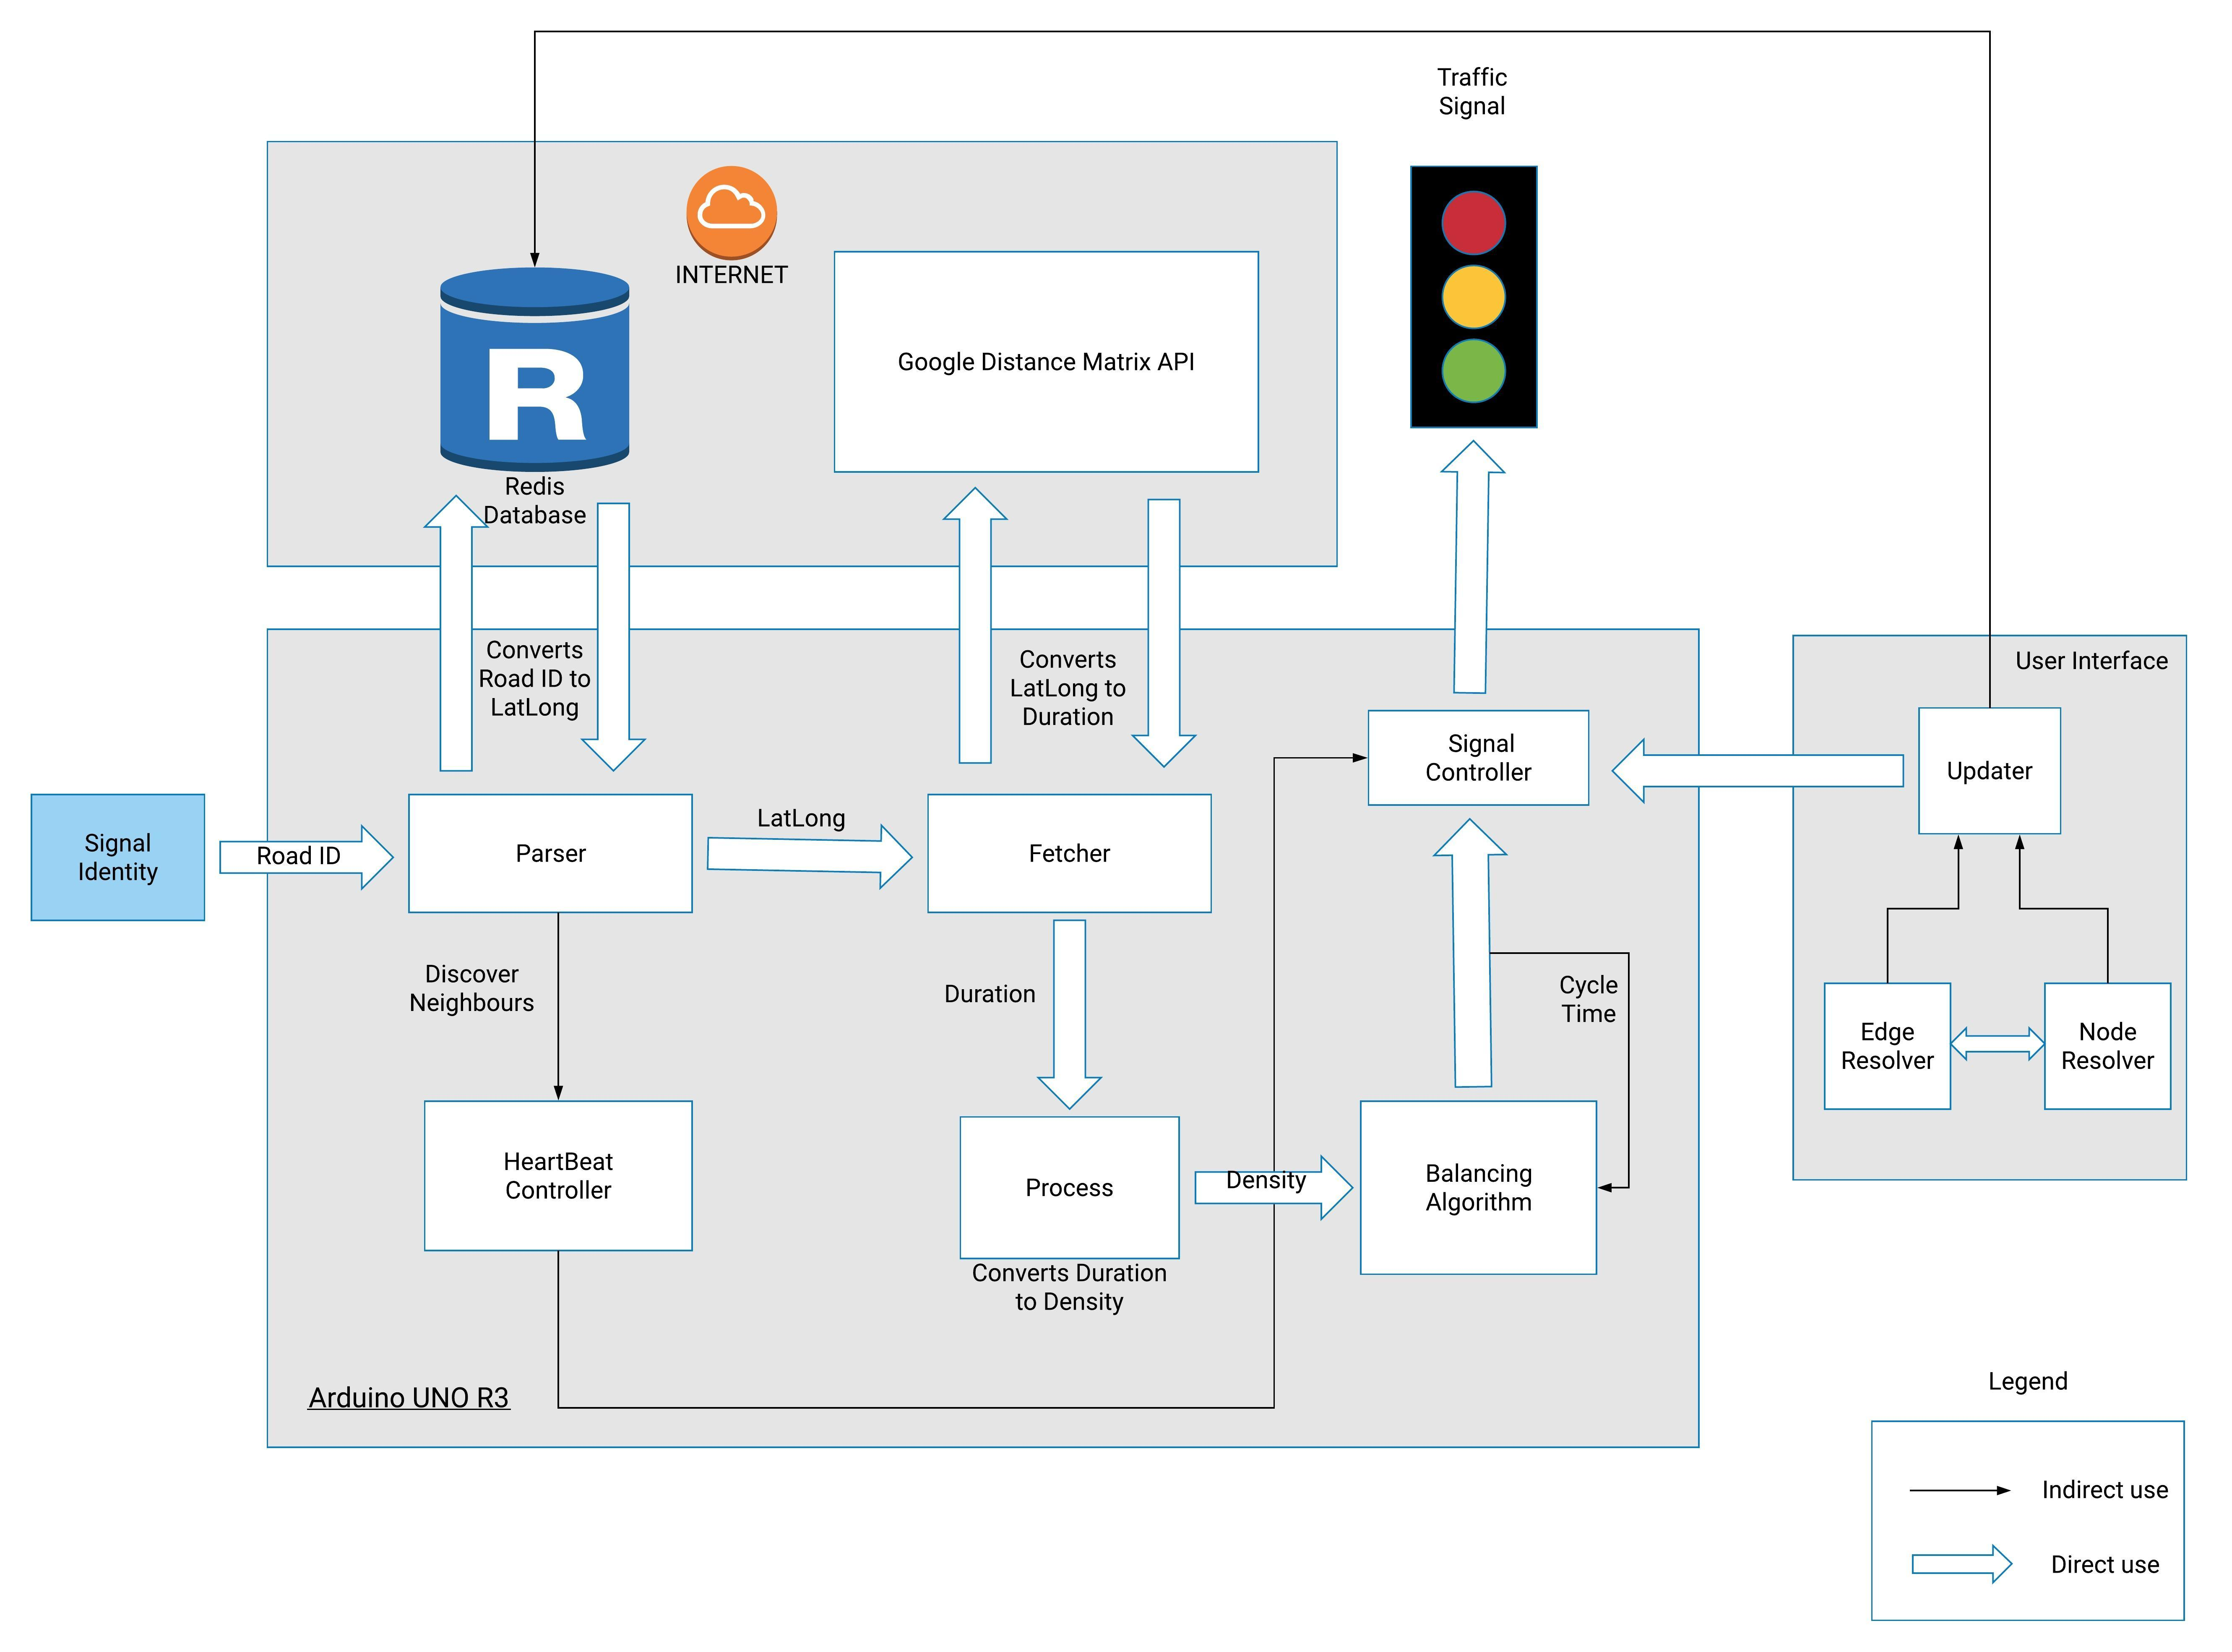
\includegraphics[scale=0.5]{Diagrams/Architecture_Diagram.jpg}
		\end{center}
		\caption{Architecture Diagram}
	\end{figure}
	
	\newpage
\subsection{Structural Diagrams}
\subsubsection{Class Diagram}
	\begin{figure}[!h]
		\begin{center}
			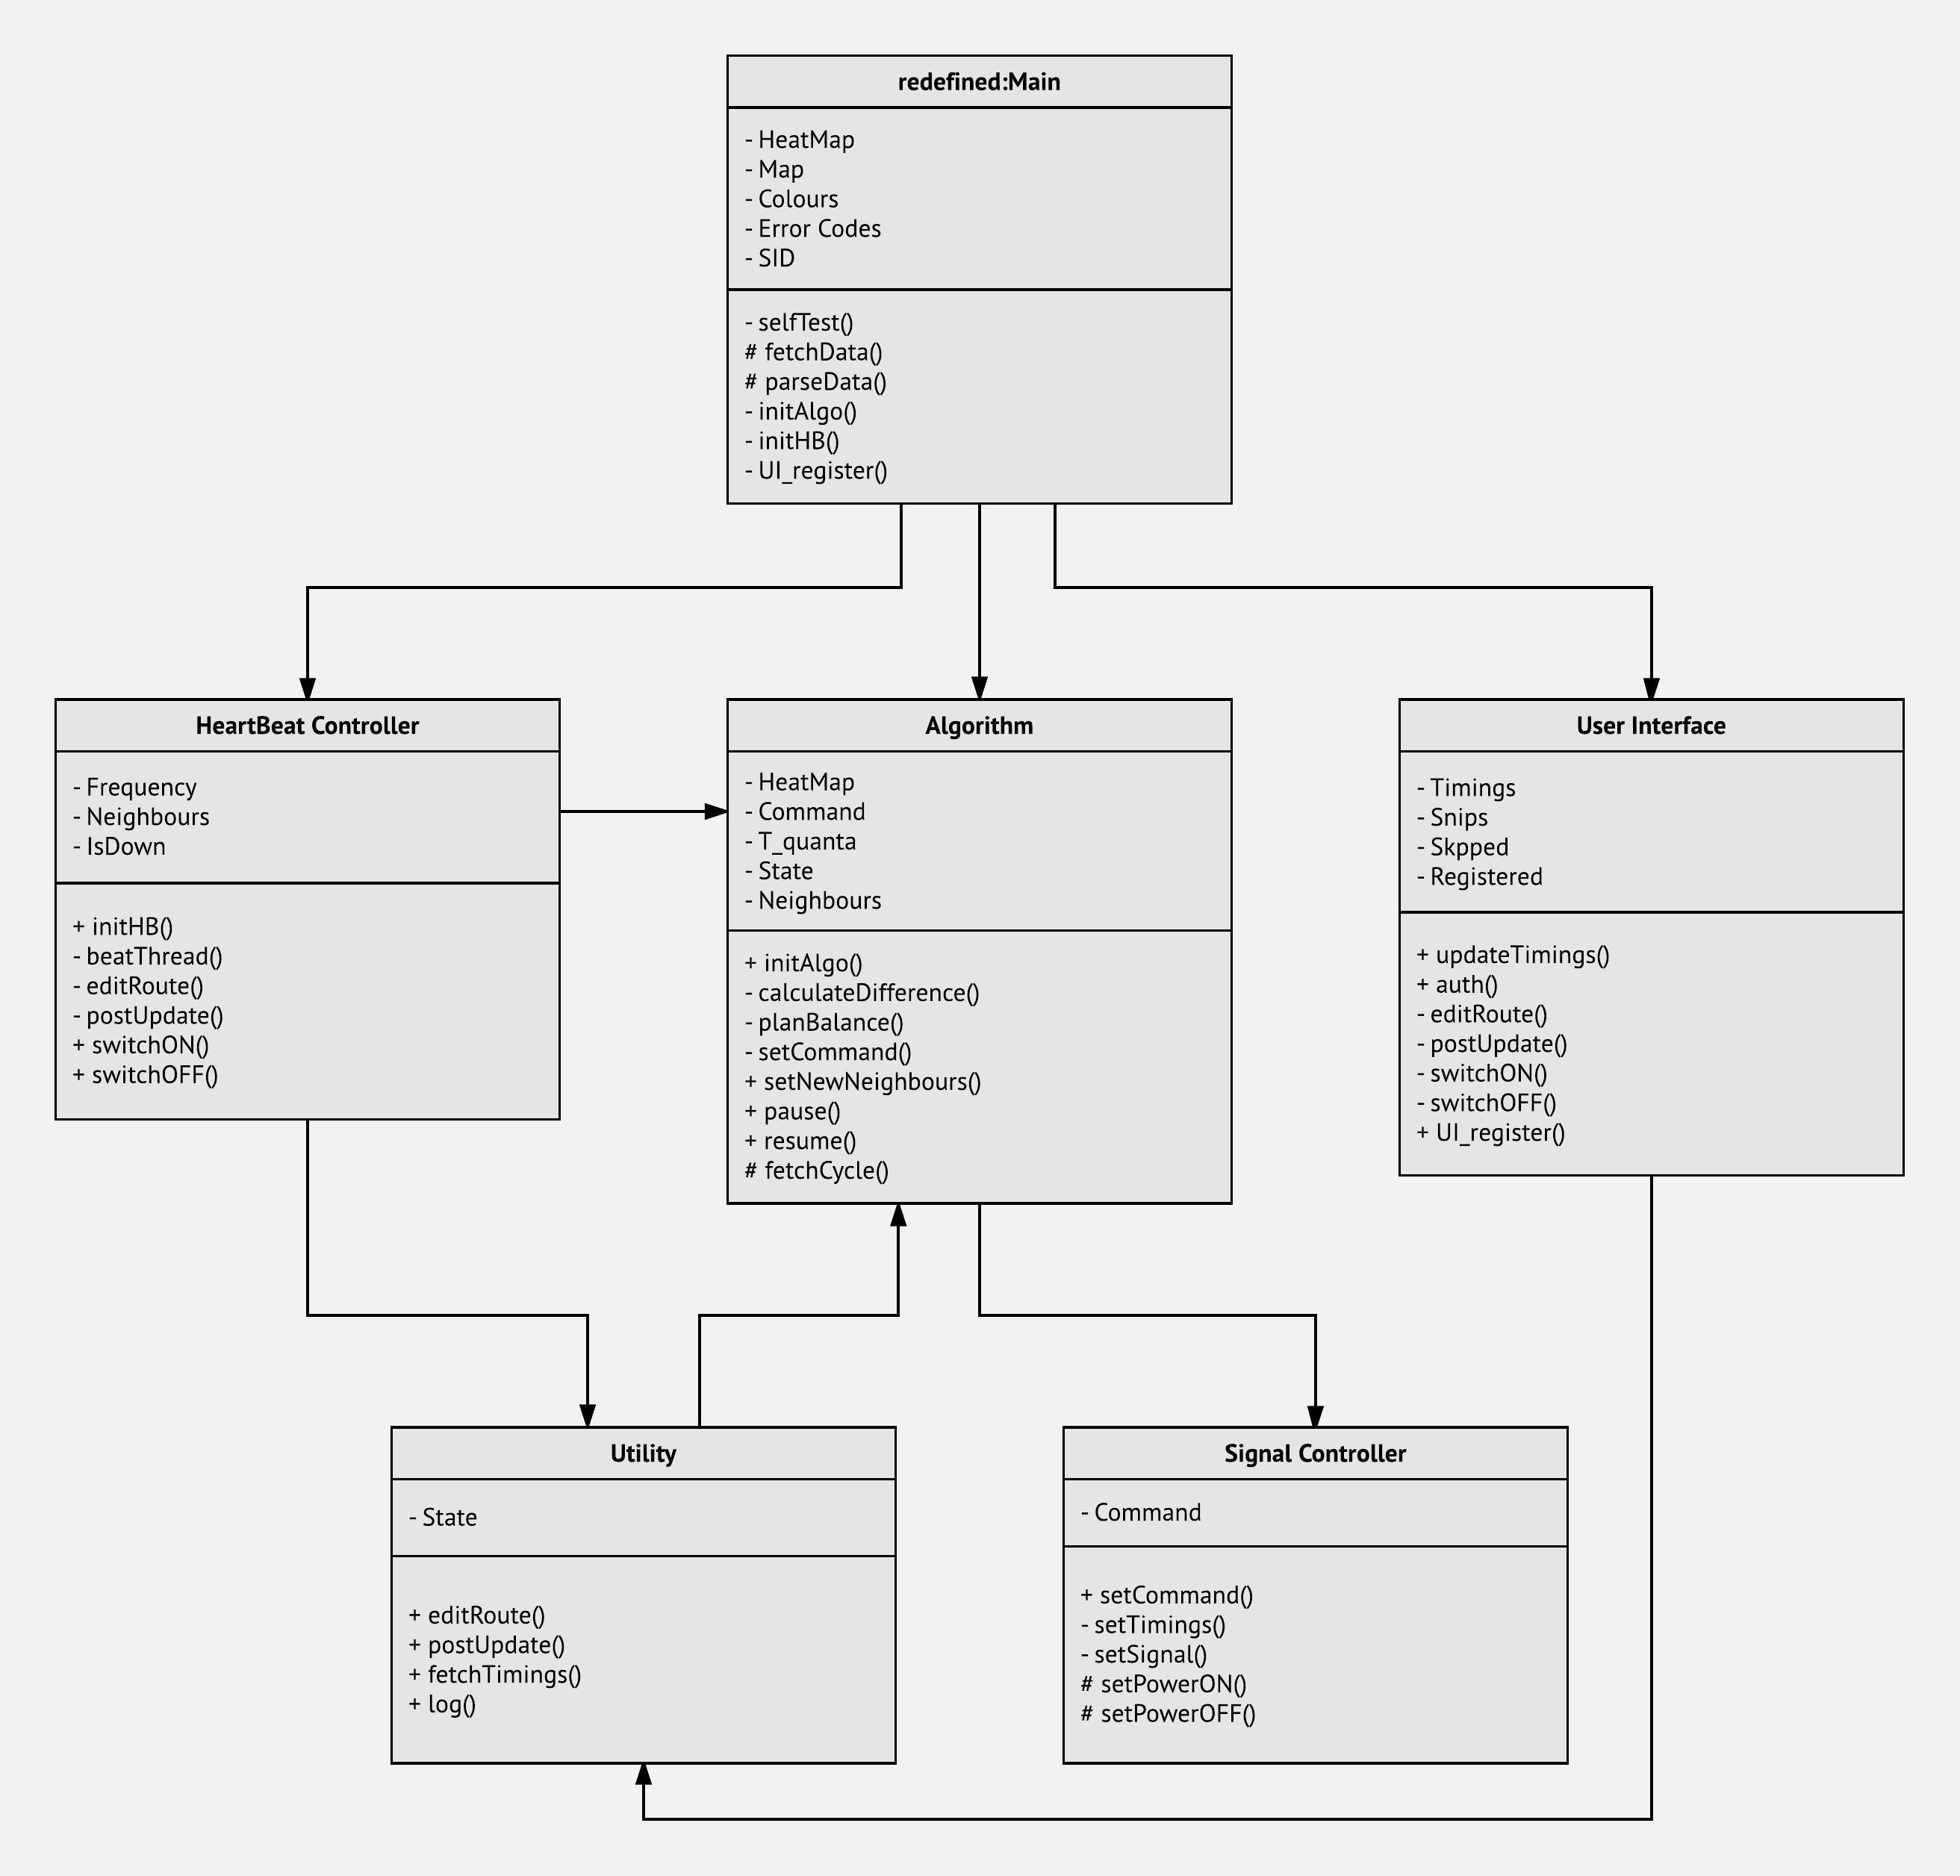
\includegraphics[scale=0.6]{Diagrams/Class_Diagram.jpeg}
		\end{center}
		\caption{Class Diagram}
	\end{figure}
\newpage
\subsubsection{Object Diagram}
	\begin{figure}[!h]
		\begin{center}
			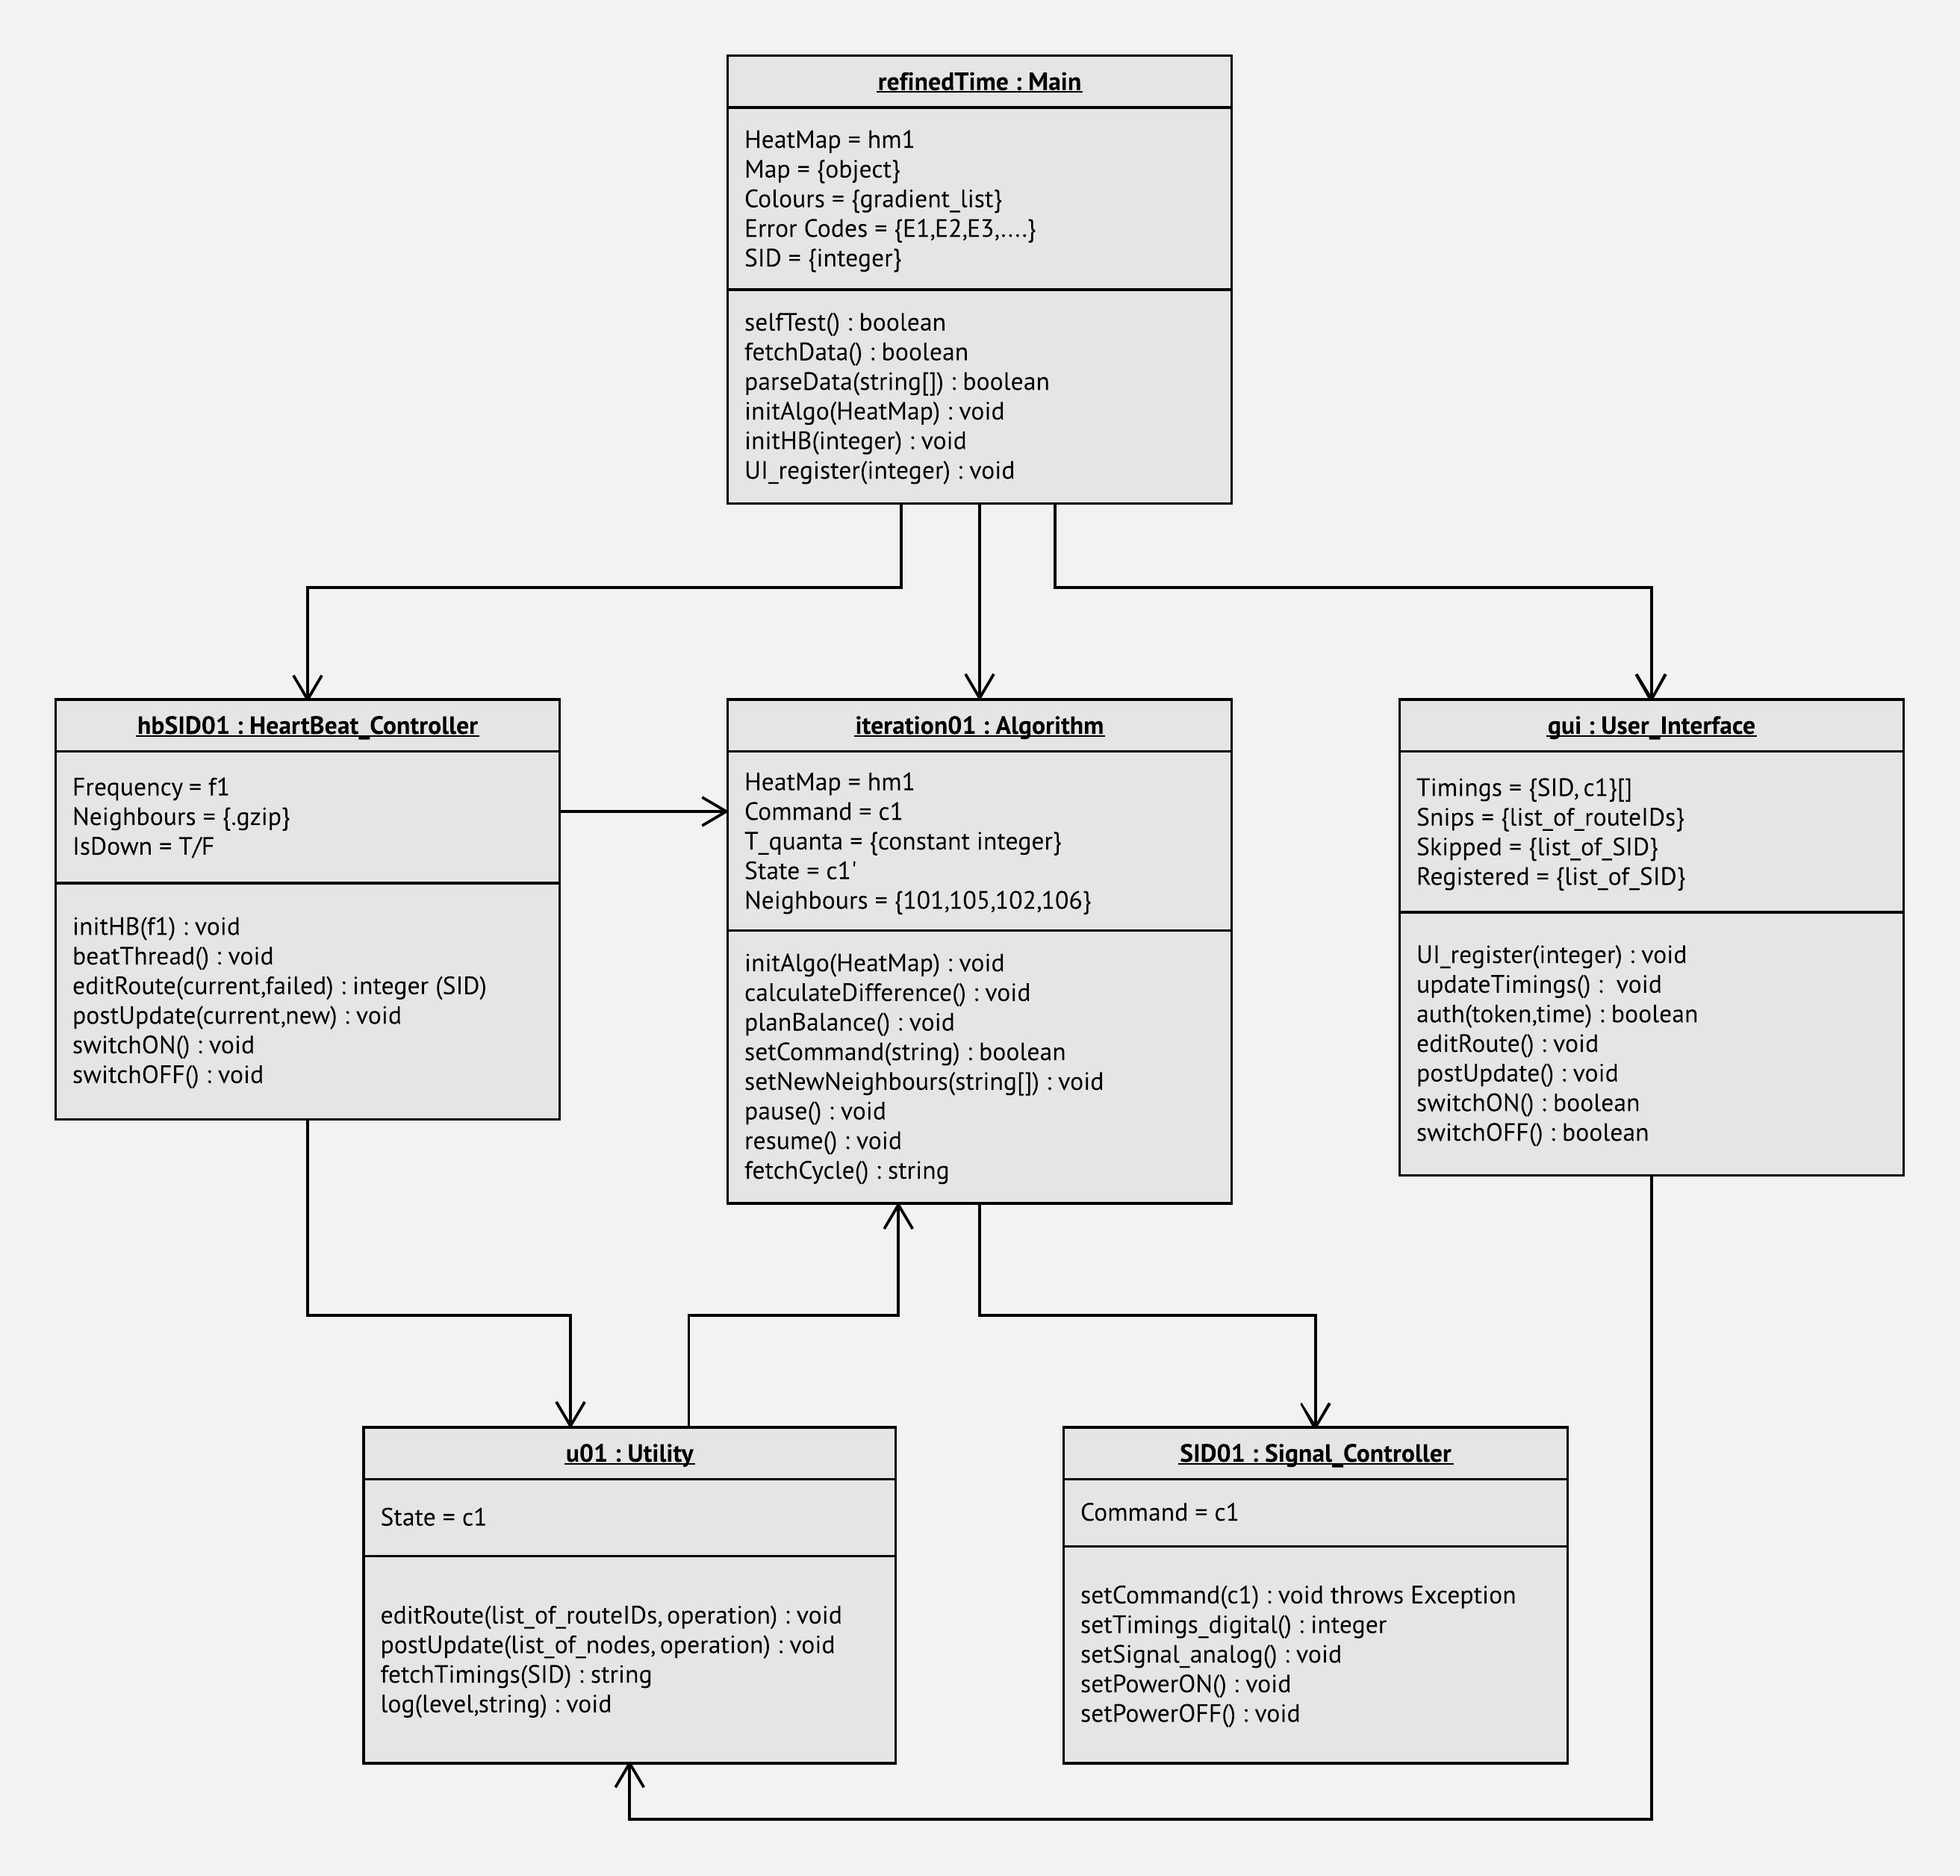
\includegraphics[scale=0.6]{Diagrams/Old Diagrams/Object_Diagram.jpeg}
		\end{center}
		\caption{Object Diagram}
	\end{figure}
\newpage
\subsubsection{Component Diagram}
	\begin{figure}[!h]
		\begin{center}
			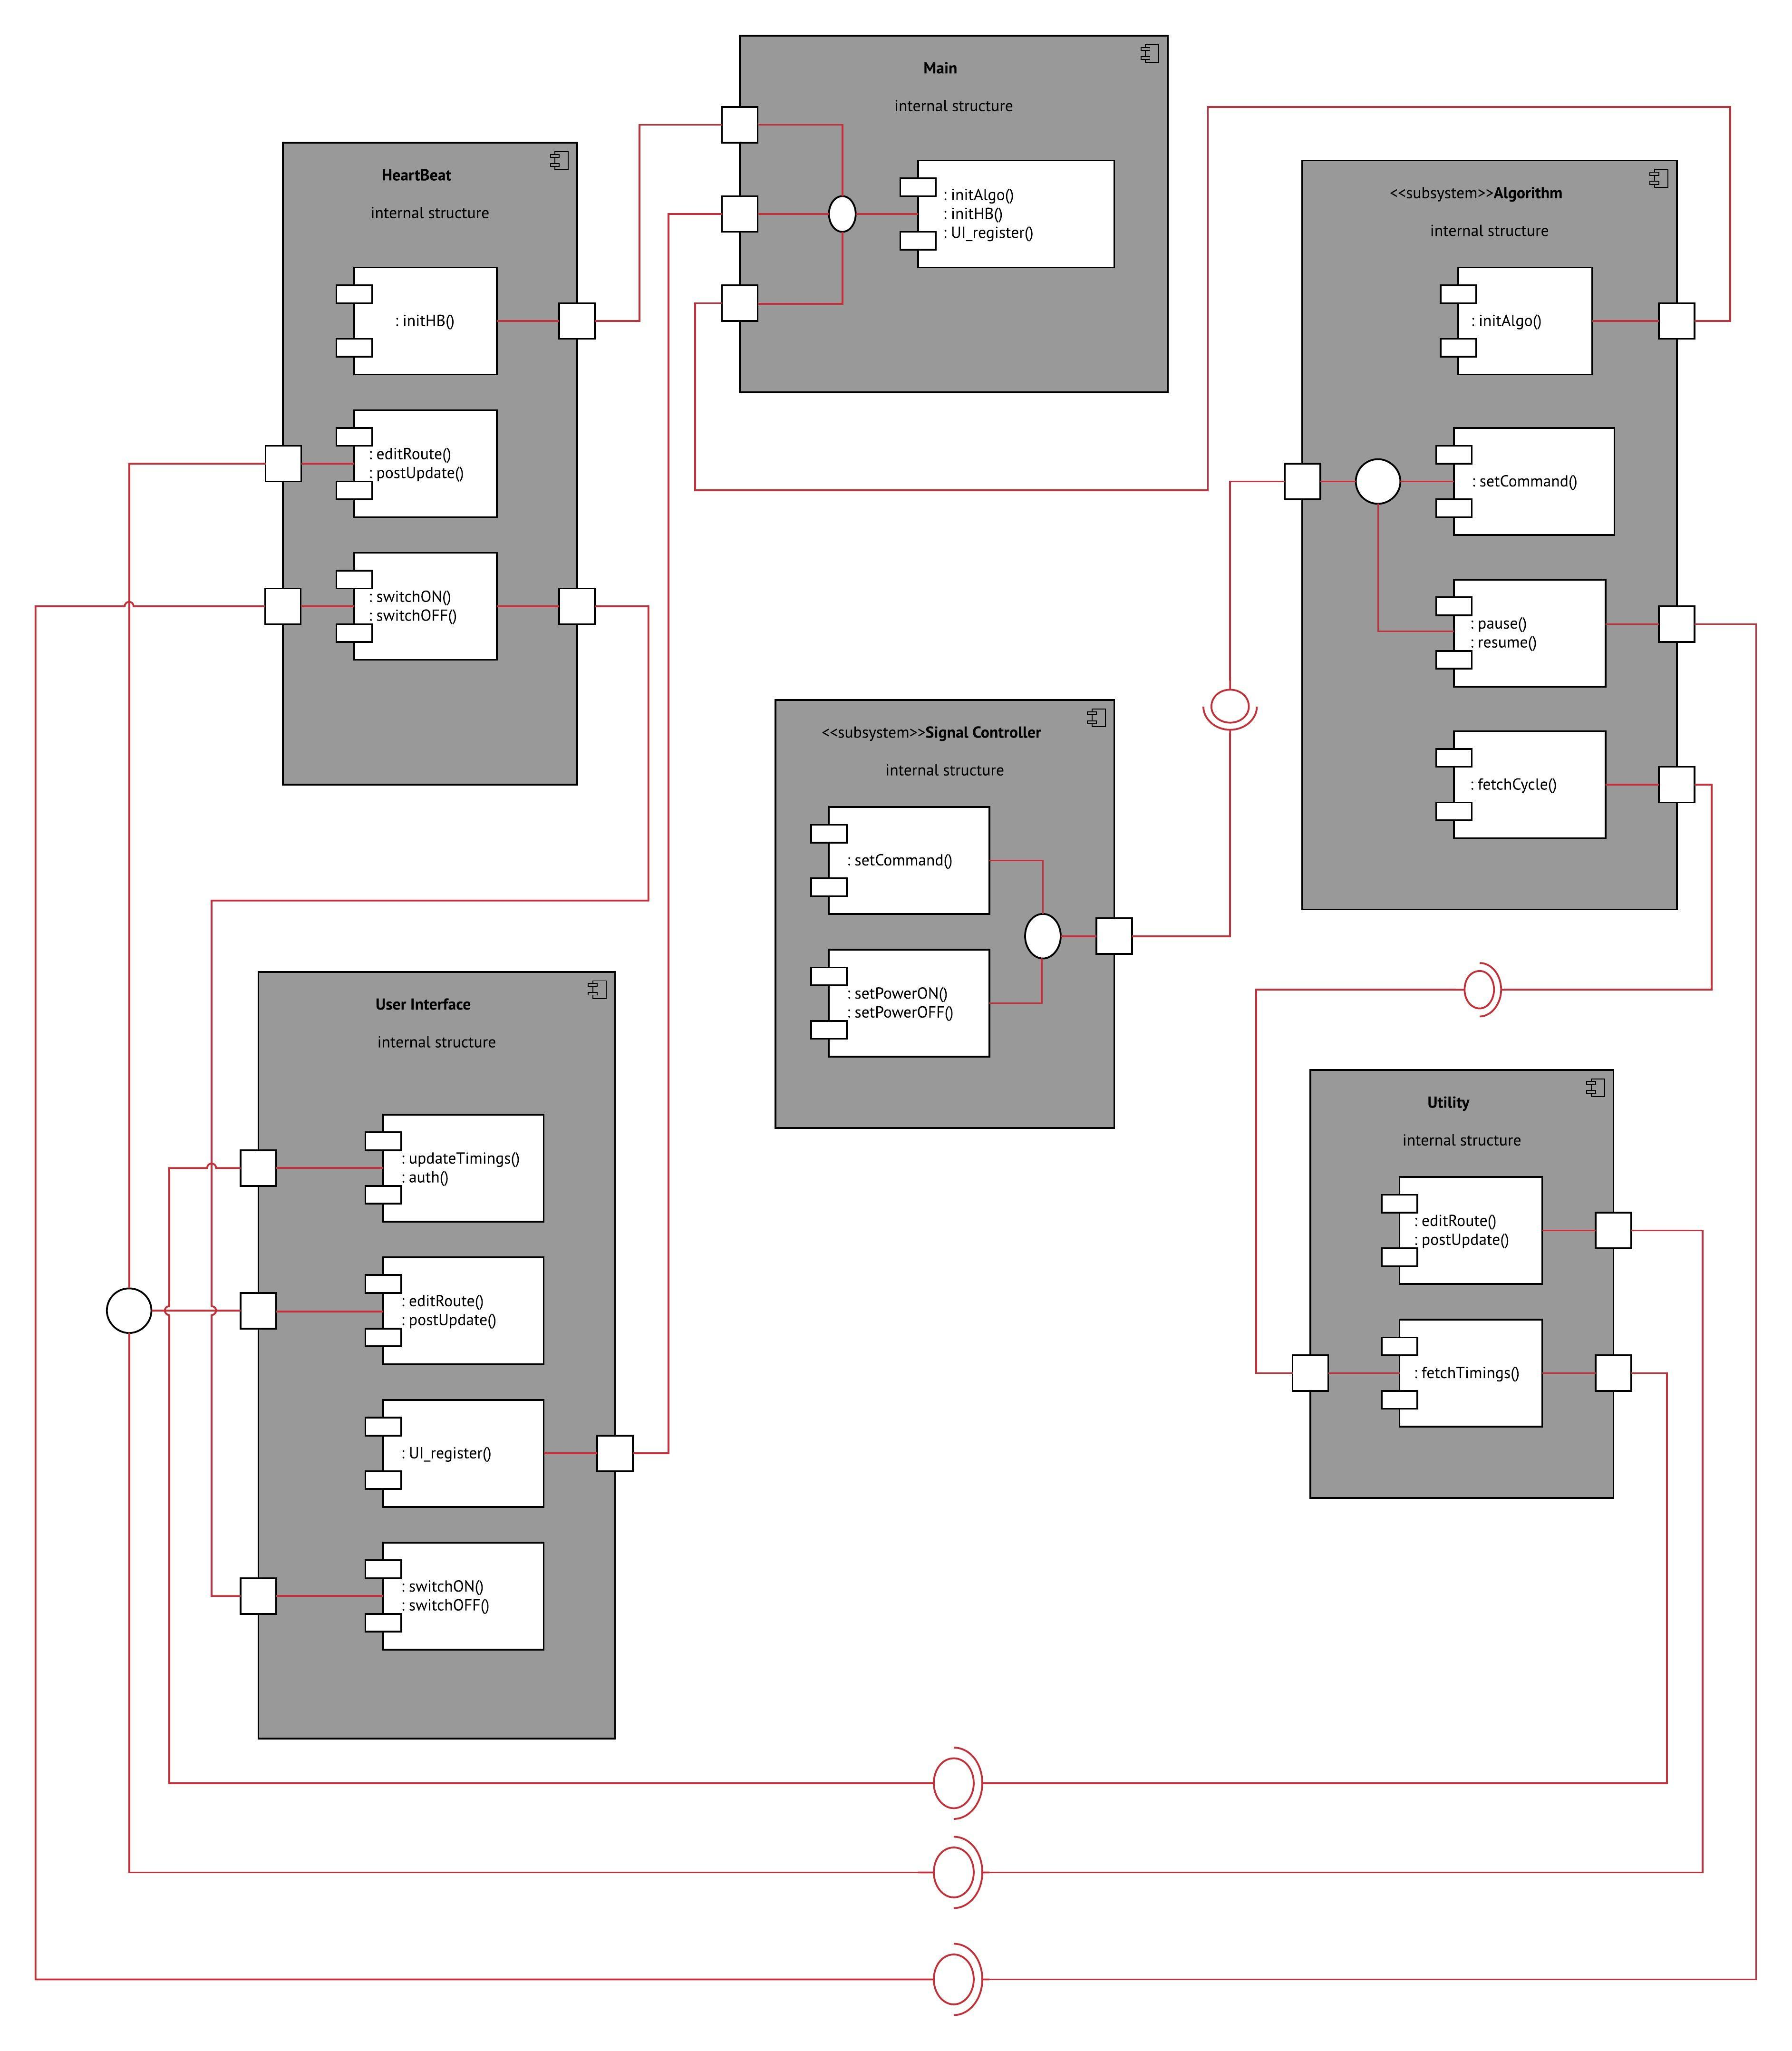
\includegraphics[scale=0.5]{Diagrams/Old Diagrams/Component_Diagram.jpeg}
		\end{center}
		\caption{Component Diagram}
	\end{figure}
\newpage
\subsection{Behavioural Diagrams}

\subsubsection{Use Case Diagram}
	\begin{figure}[!h]
		\begin{center}
			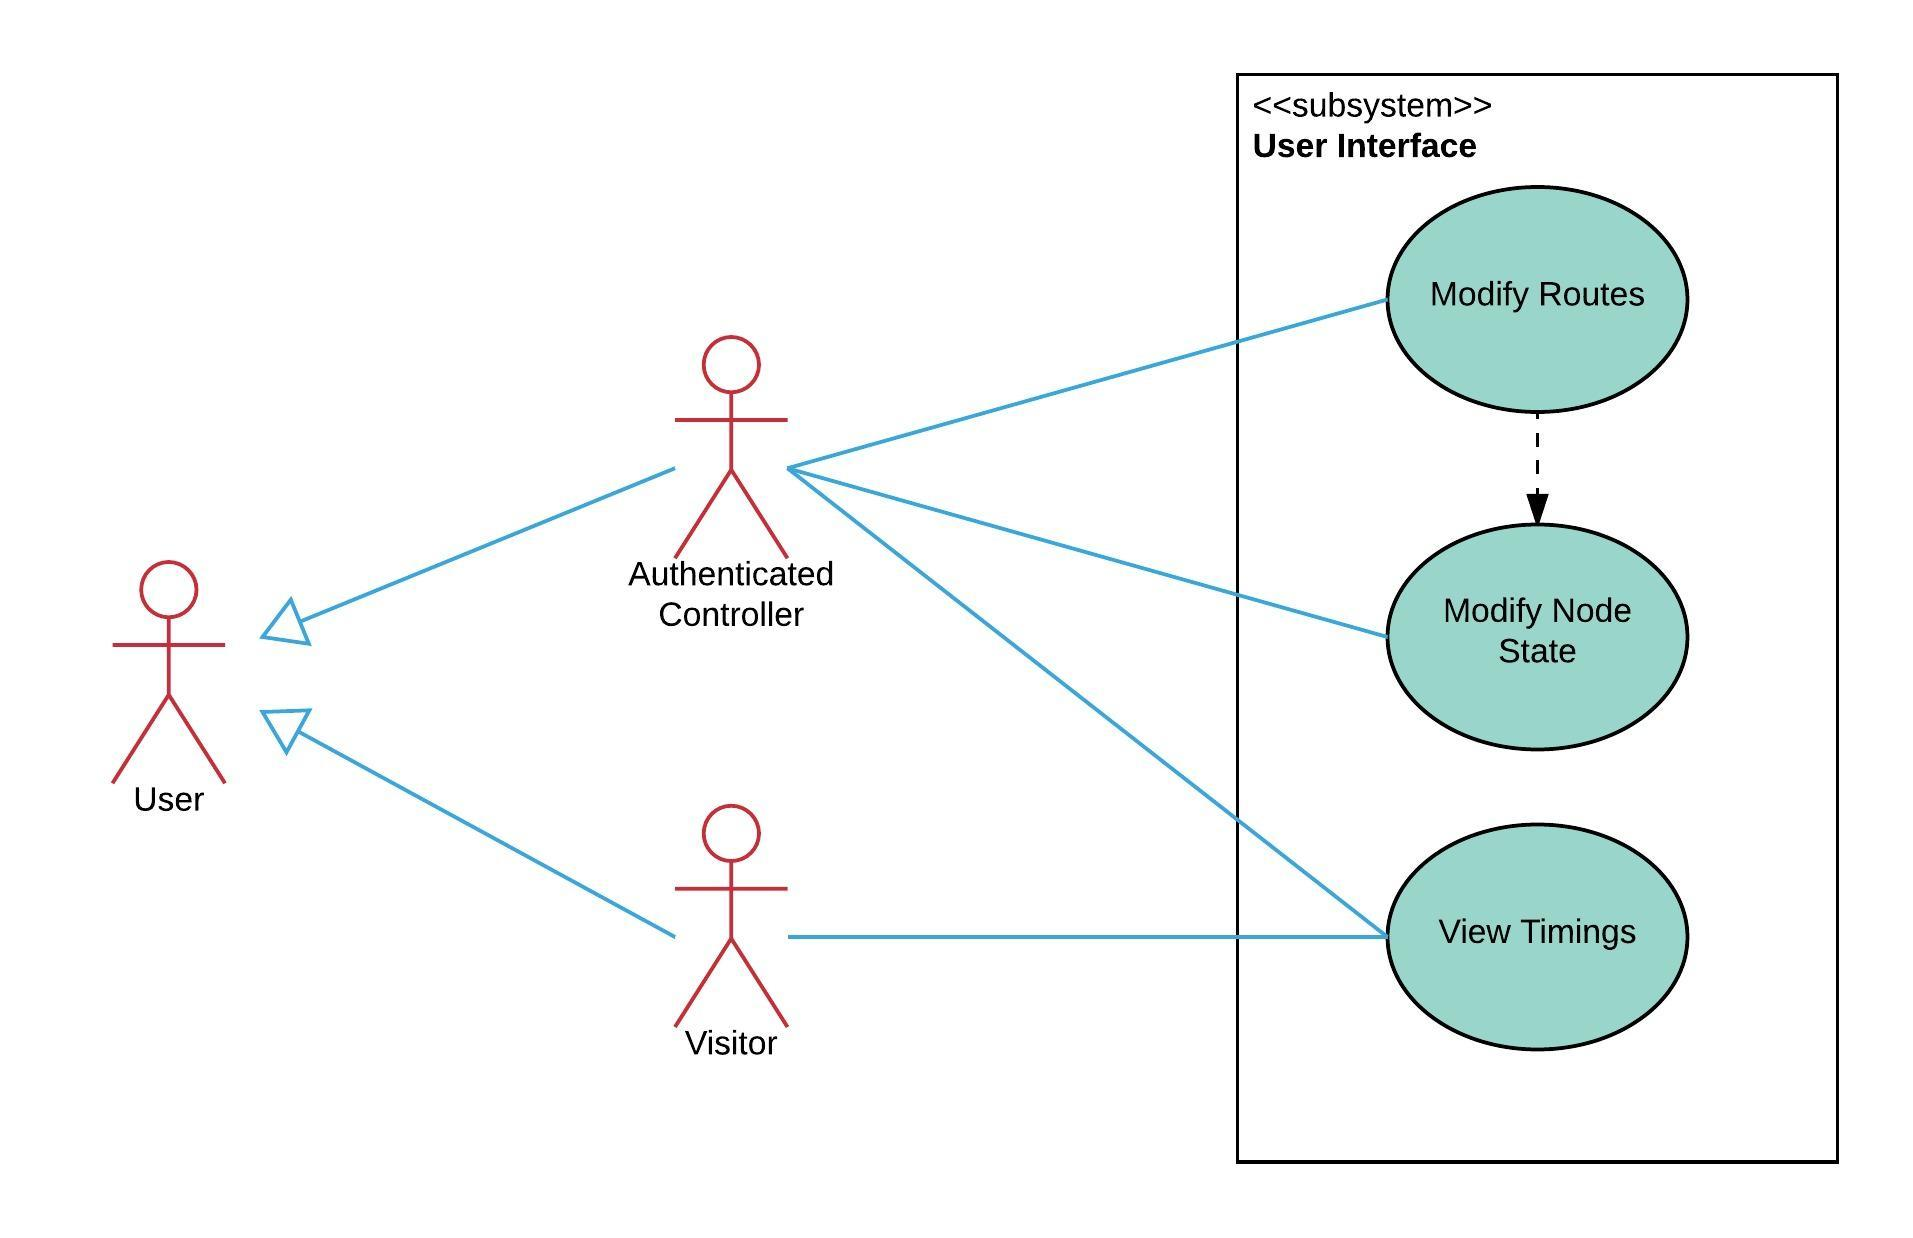
\includegraphics[scale=0.2]{Diagrams/Old Diagrams/Use_Case_Diagram.jpeg}
		\end{center}
		\caption{Use Case Diagram}
	\end{figure}
	
\subsubsection{StateChart Diagram}
	\begin{figure}[!h]
		\begin{center}
			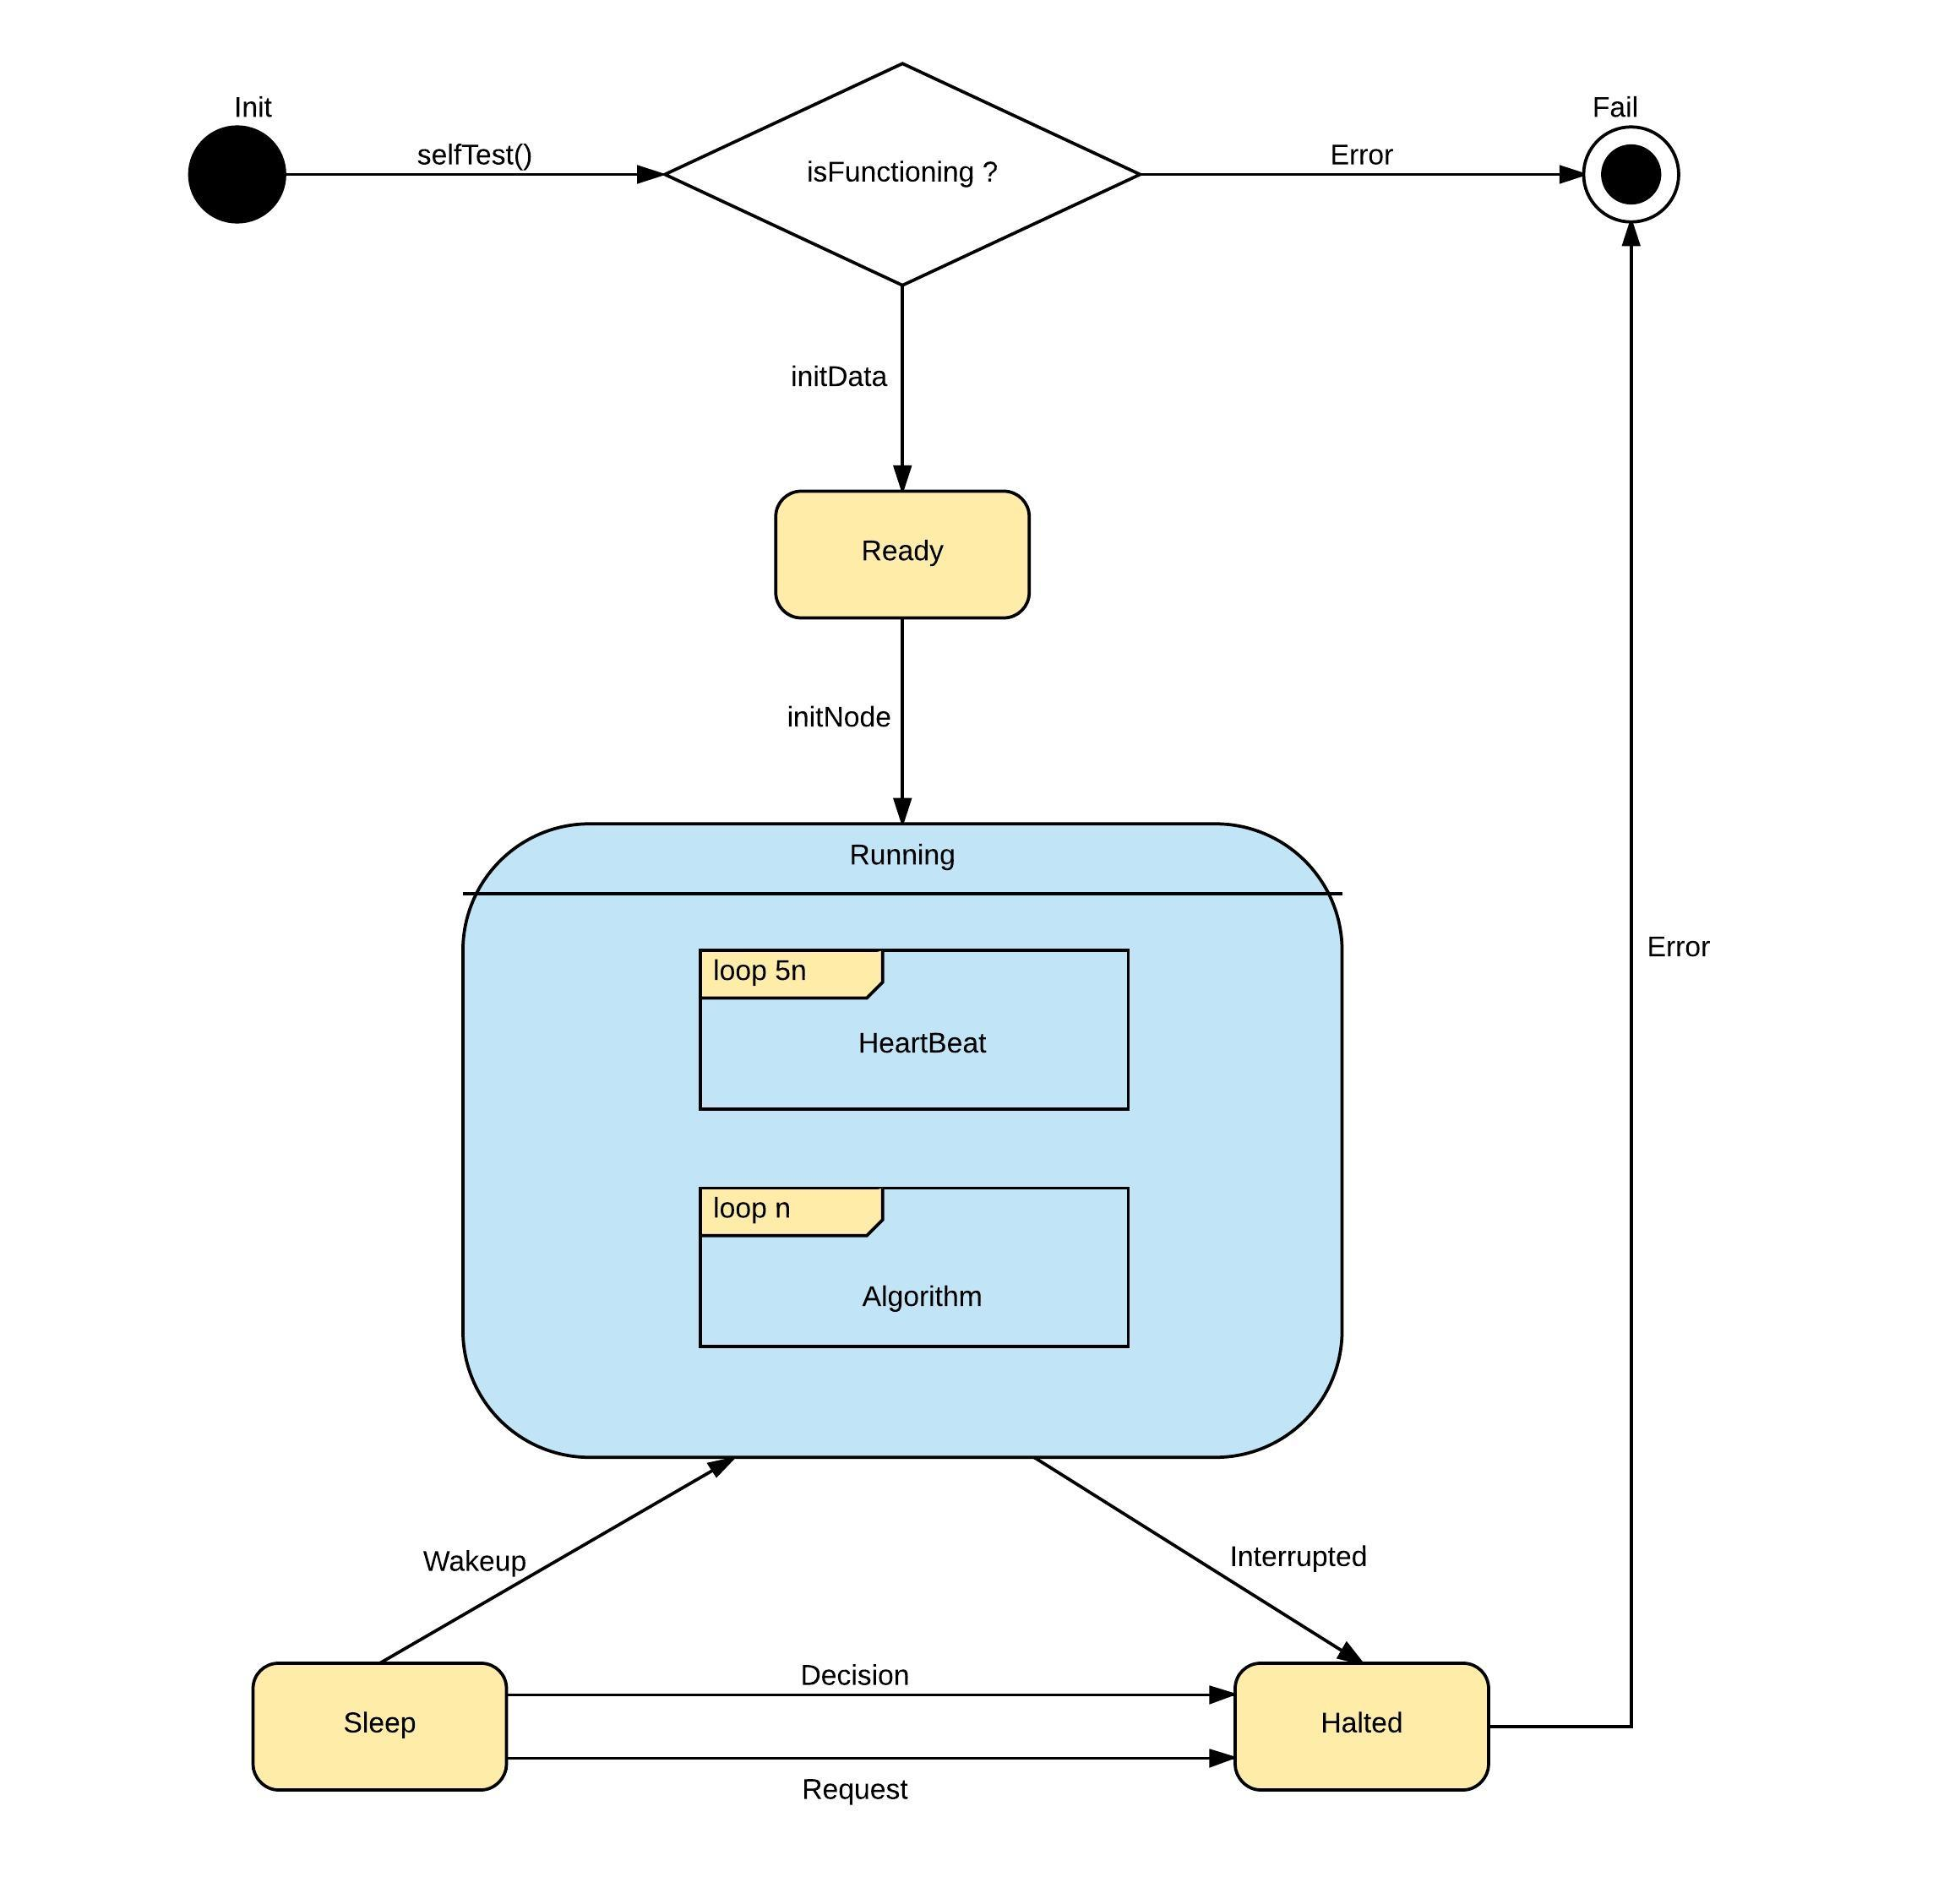
\includegraphics[scale=0.12]{Diagrams/Old Diagrams/StateChart_Diagram.jpeg}
		\end{center}
		\caption{StateChart Diagram}
	\end{figure}

\subsubsection{Sequence Diagrams}
	\begin{figure}[!h]
		\begin{center}
			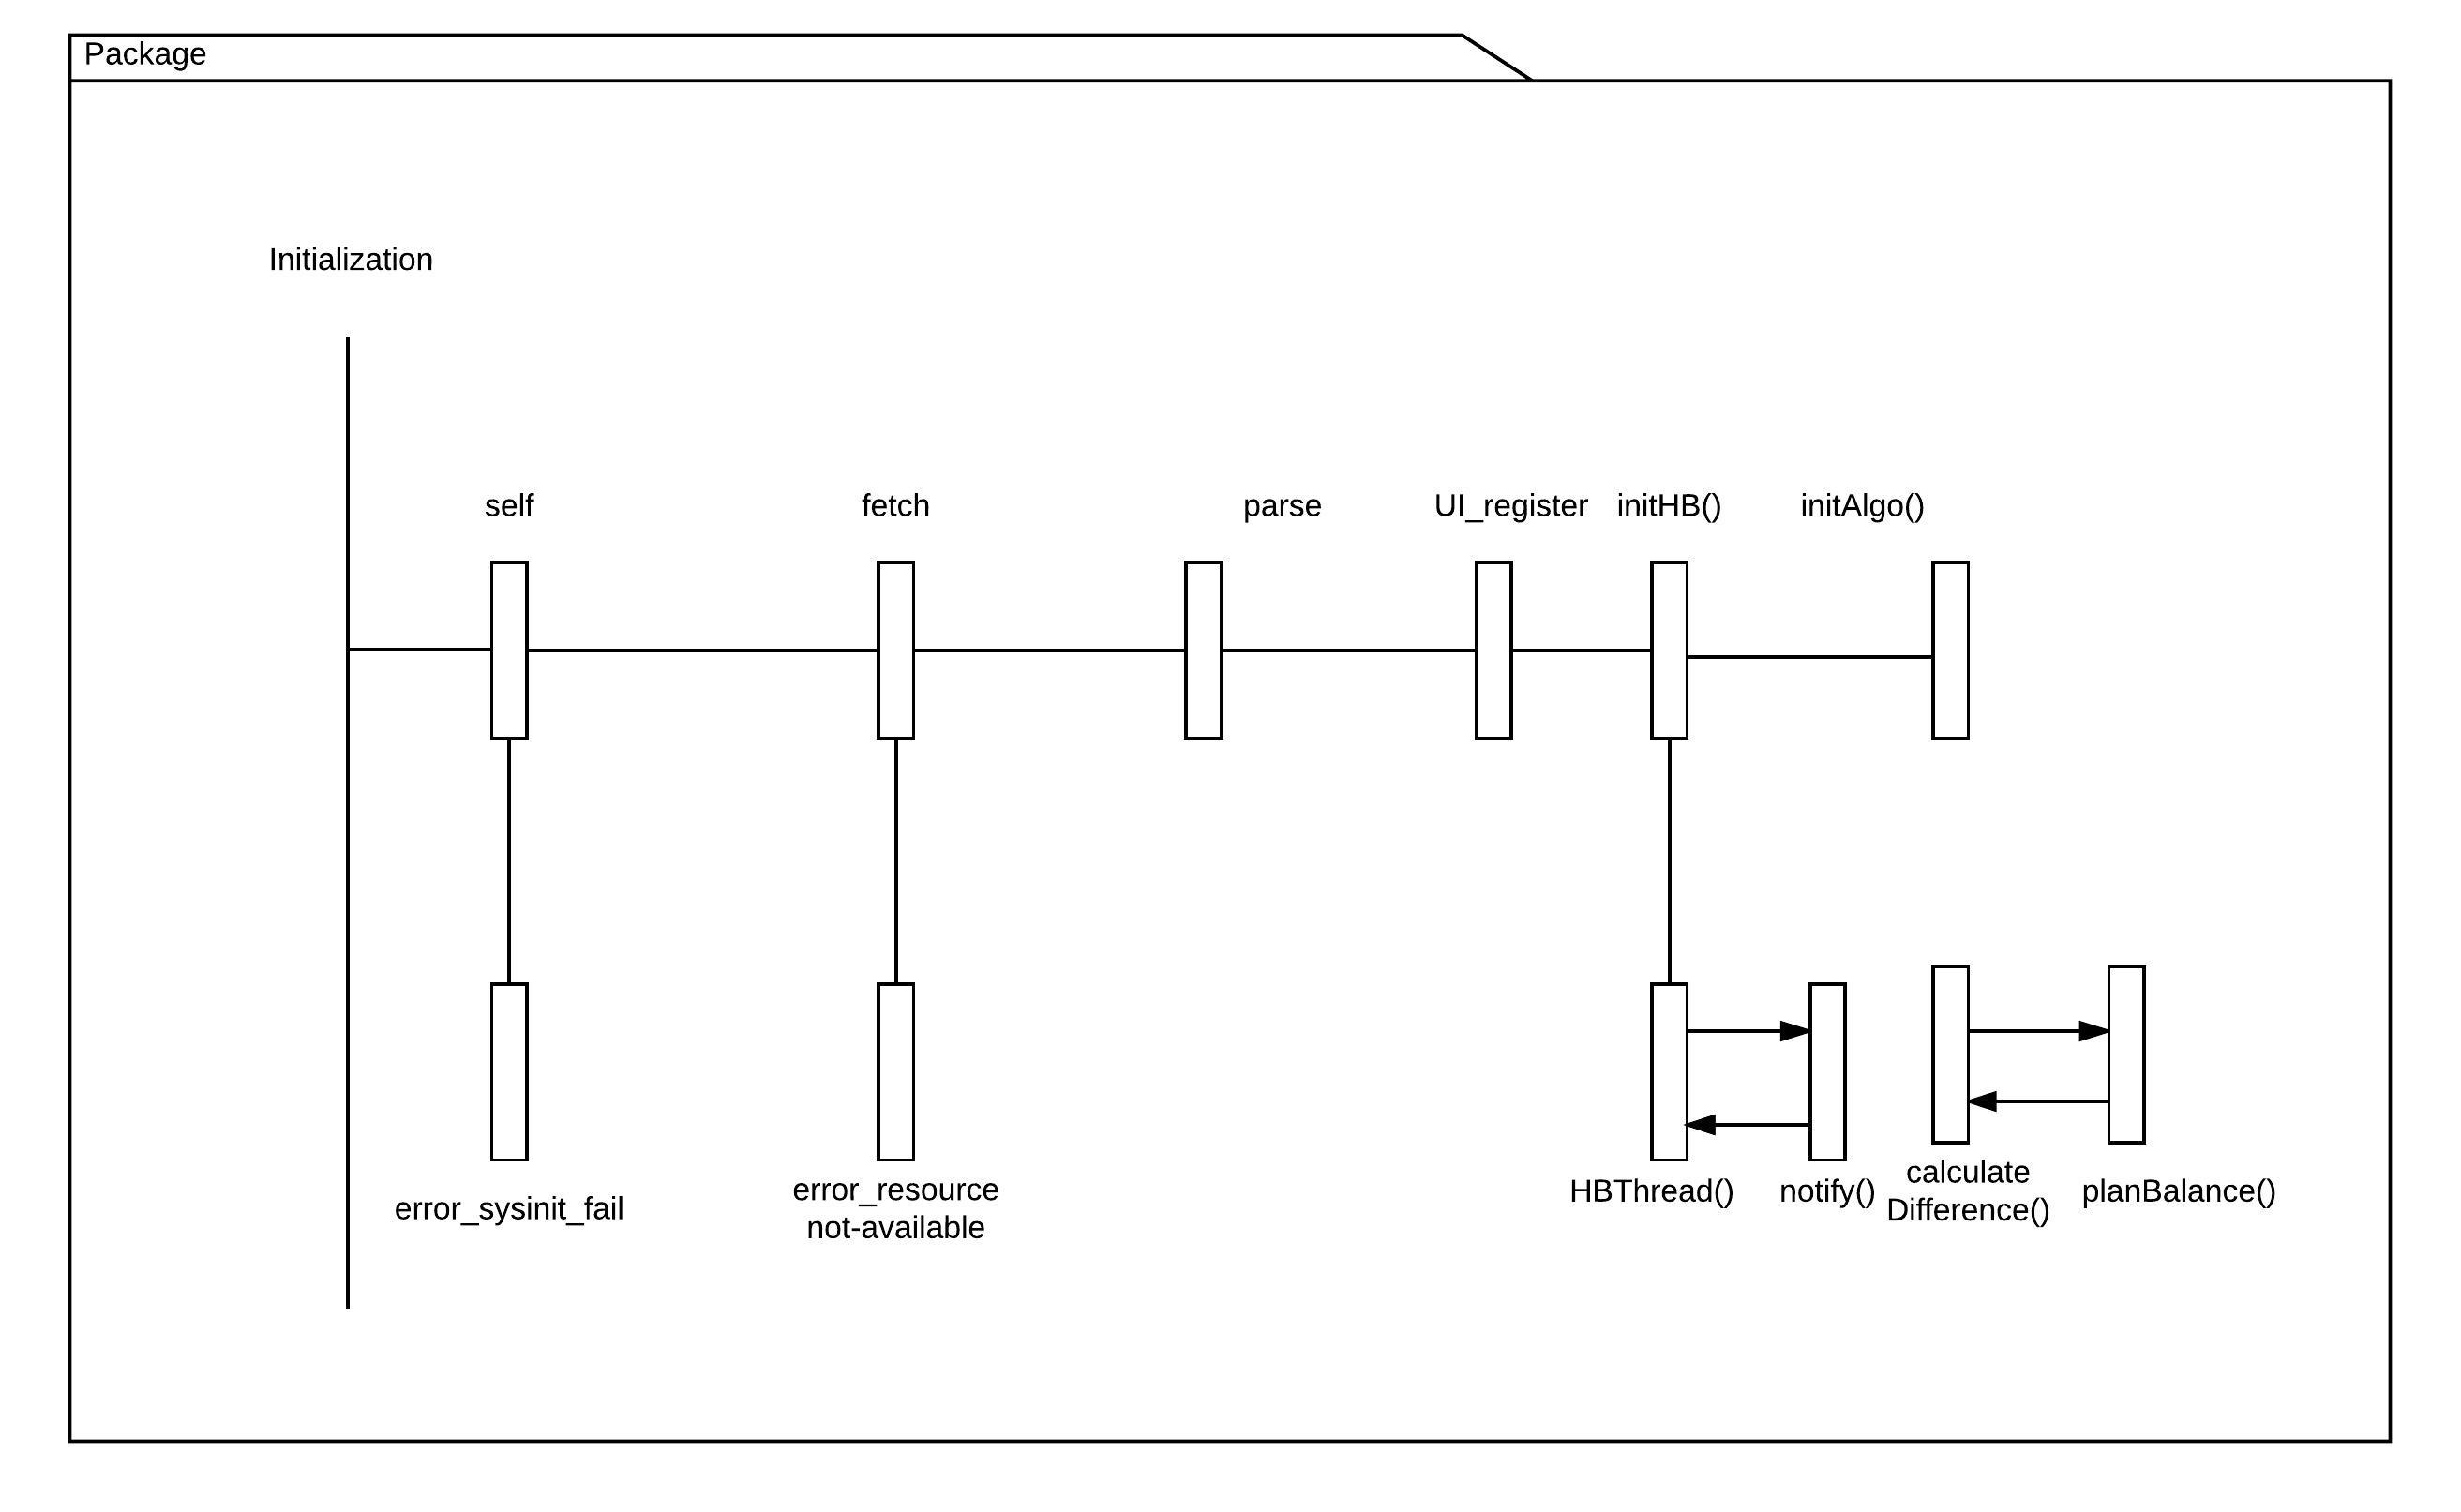
\includegraphics[scale=0.6]{Diagrams/Old Diagrams/First_Sequence.jpeg}
		\end{center}
		\caption{Initialization Sequence}
	\end{figure}
	\begin{figure}[!h]
		\begin{center}
			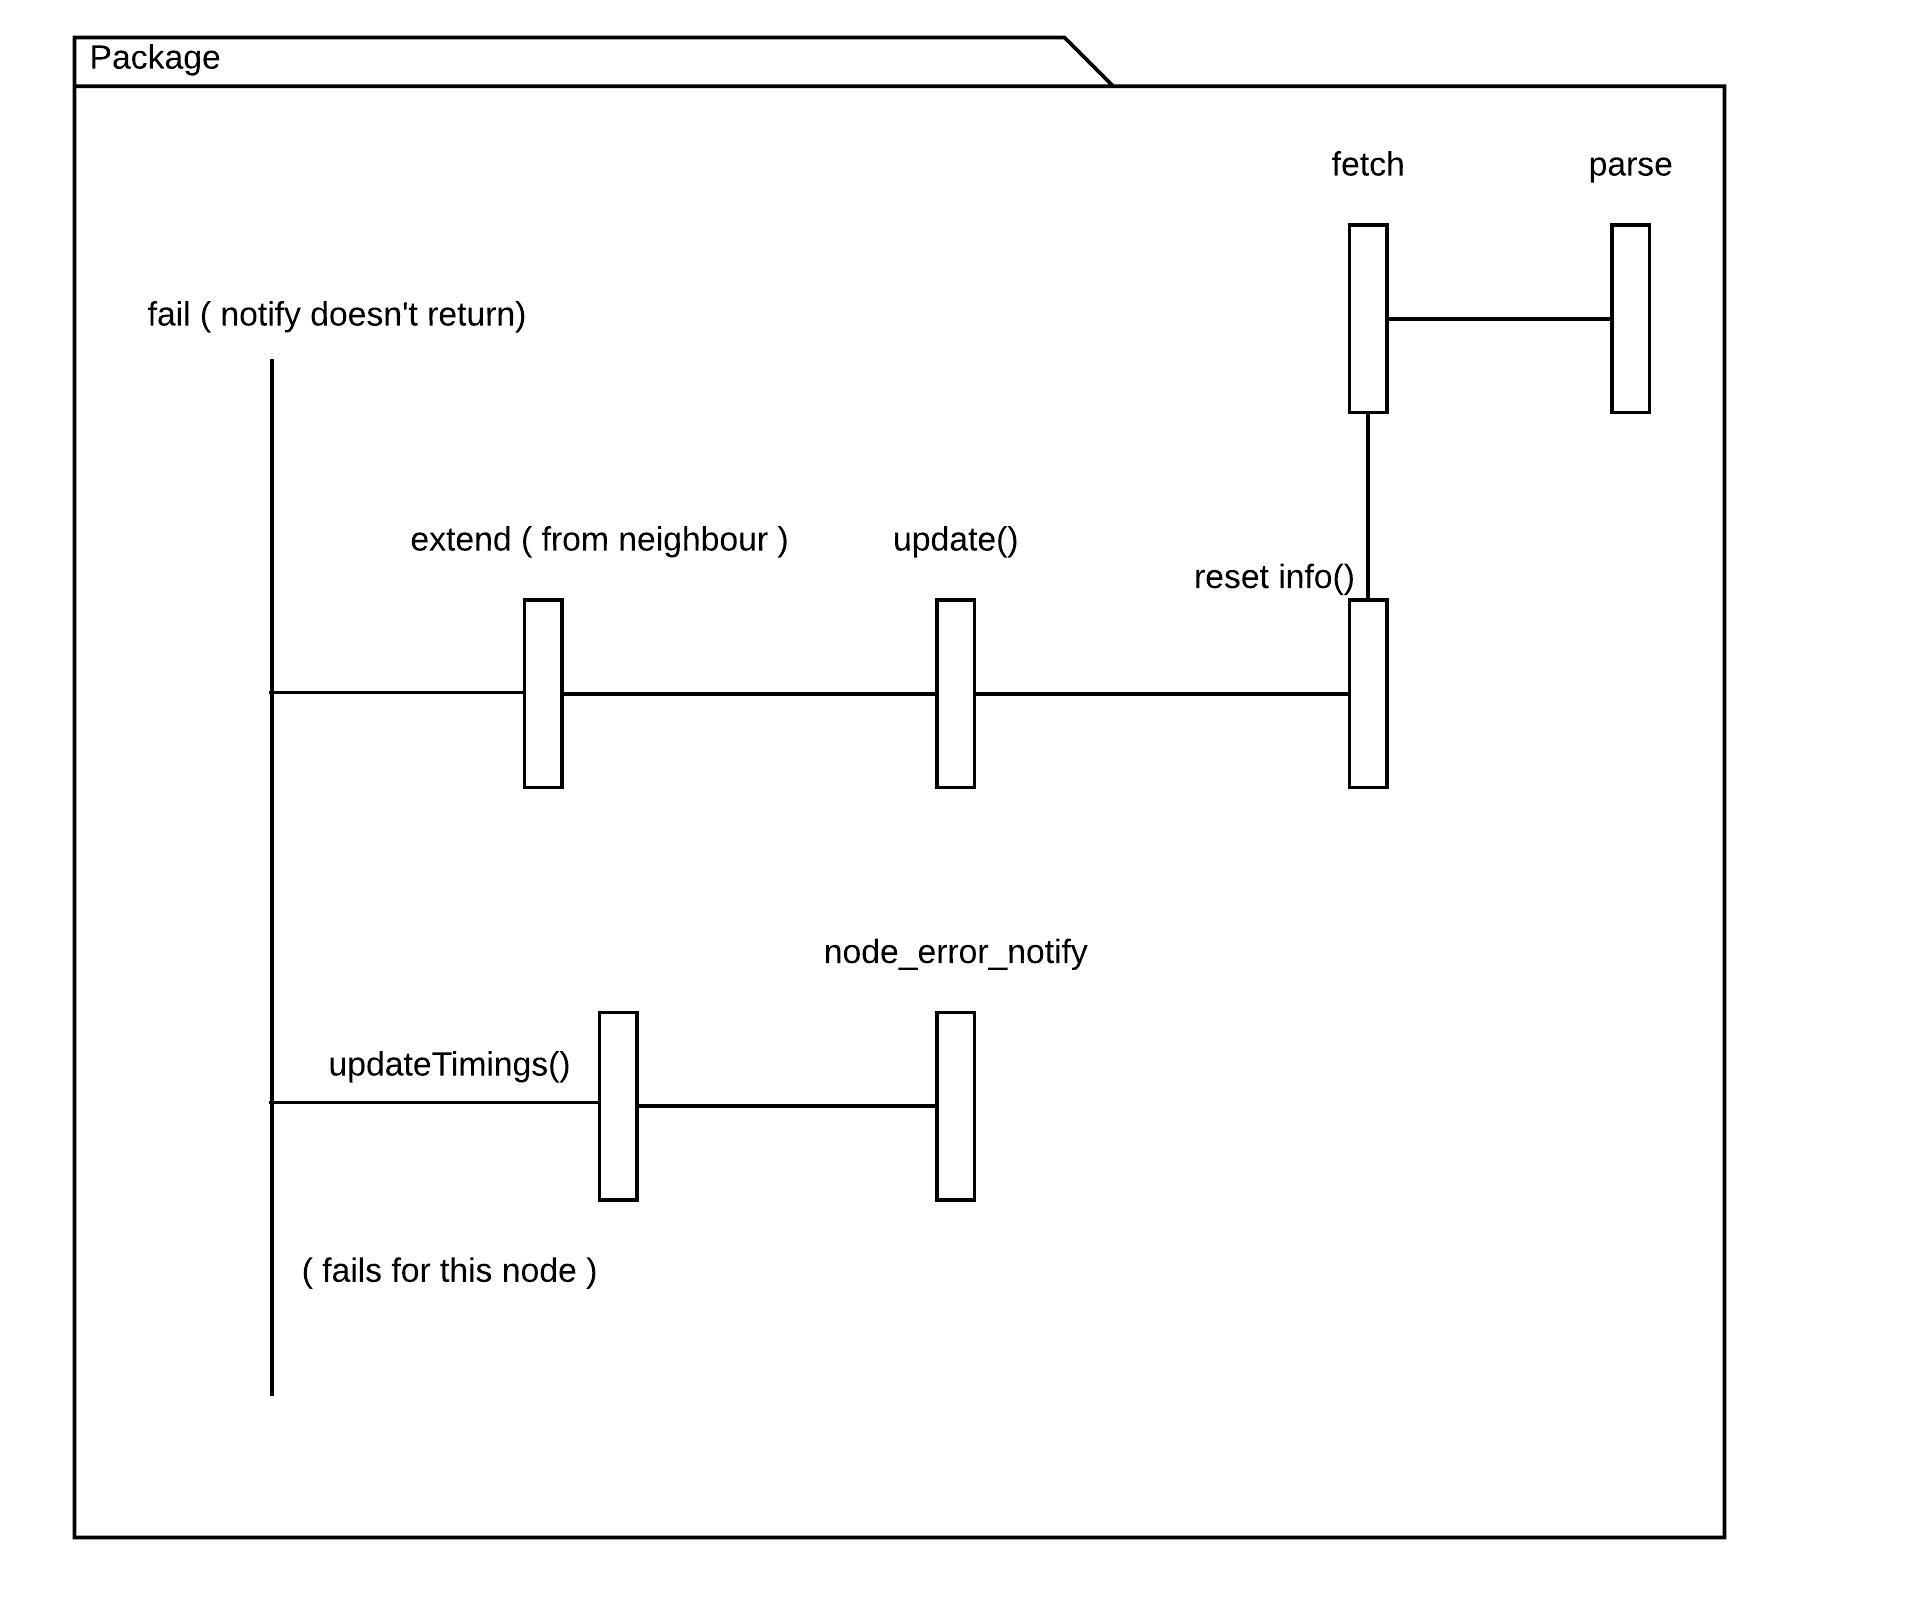
\includegraphics[scale=0.6]{Diagrams/Old Diagrams/Error_Sequence.jpeg}
		\end{center}
		\caption{Sequence for Failure of a Node}
	\end{figure}
	\begin{figure}[!h]
		\begin{center}
			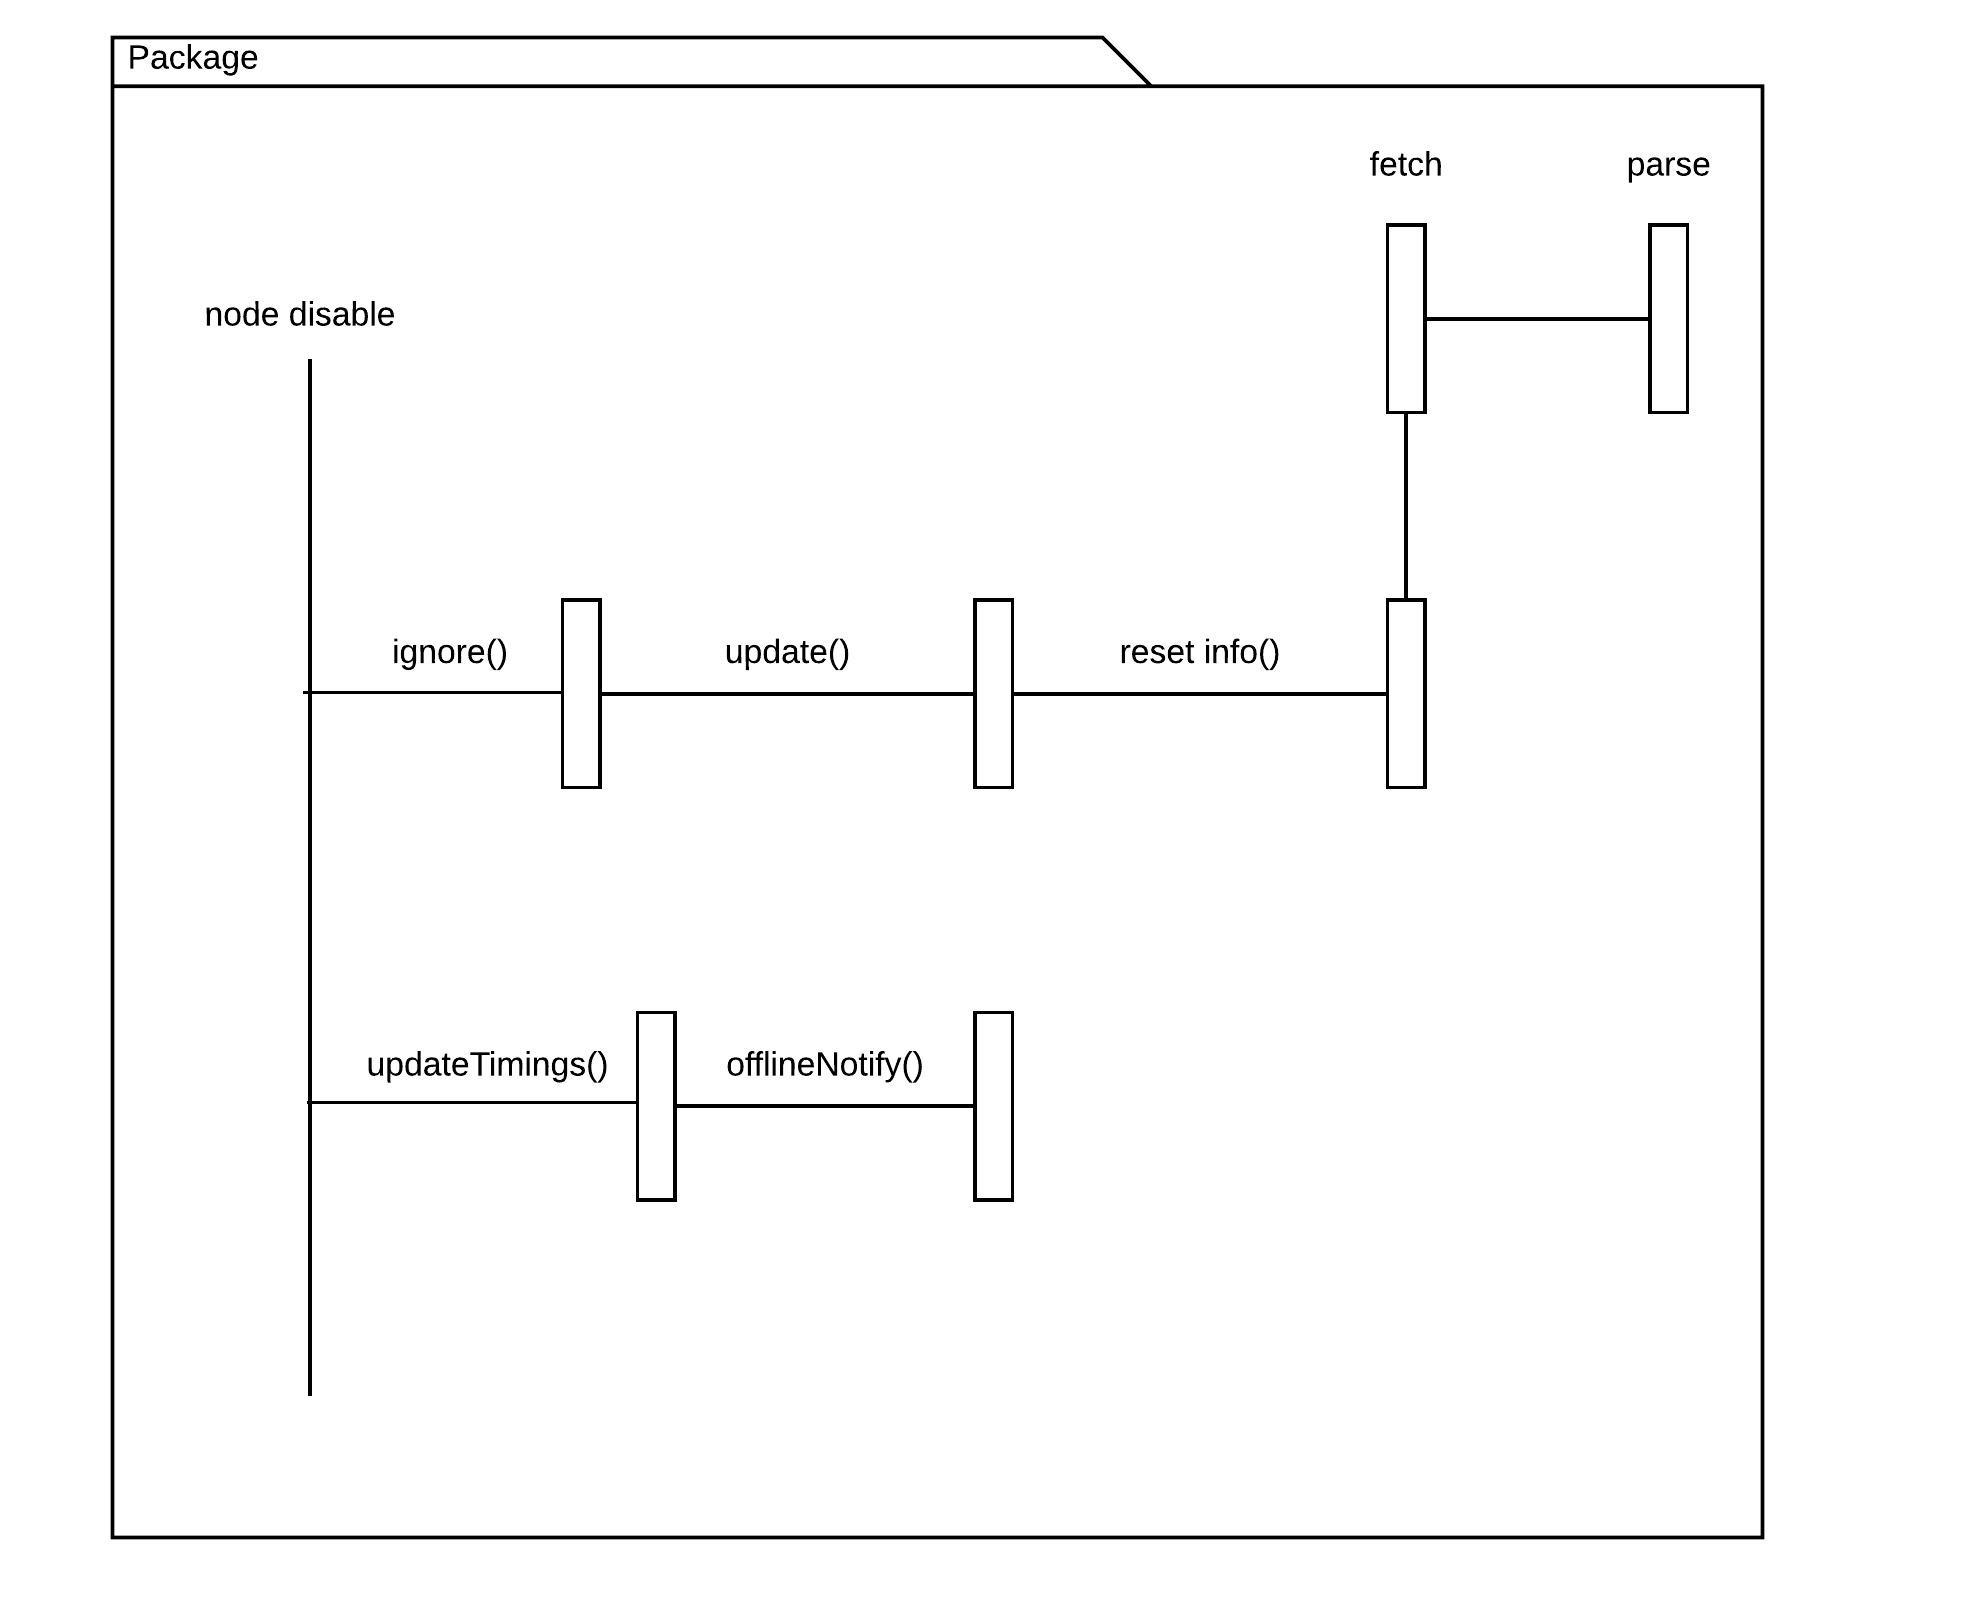
\includegraphics[scale=0.6]{Diagrams/Old Diagrams/Node_Disable_Sequence.jpeg}
		\end{center}
		\caption{Node Removal Sequence}
	\end{figure}
	\begin{figure}[!h]
		\begin{center}
			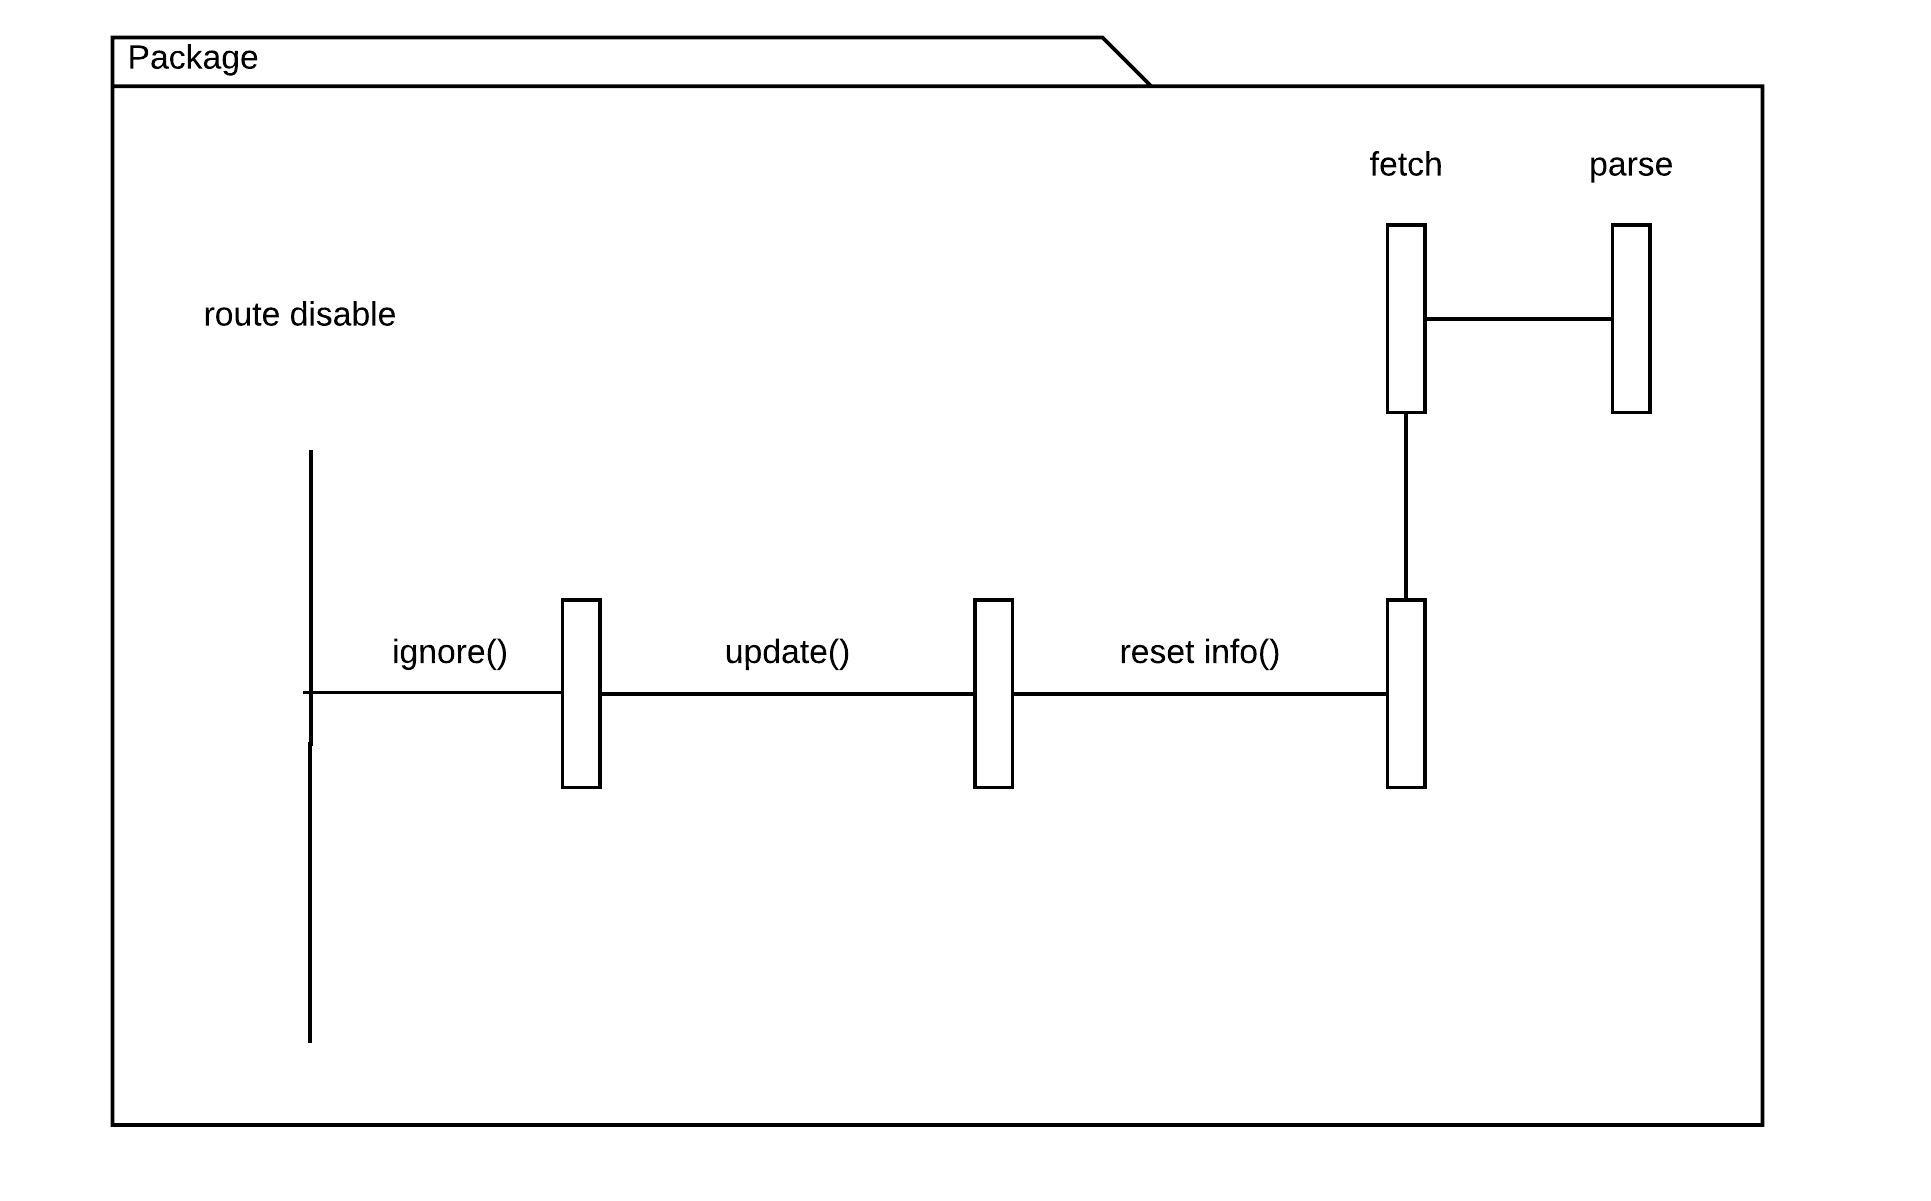
\includegraphics[scale=0.6]{Diagrams/Old Diagrams/Route_Disable_Sequence.jpeg}
		\end{center}
		\caption{Route Modification Sequence}
	\end{figure}
	\begin{figure}[!h]
		\begin{center}
			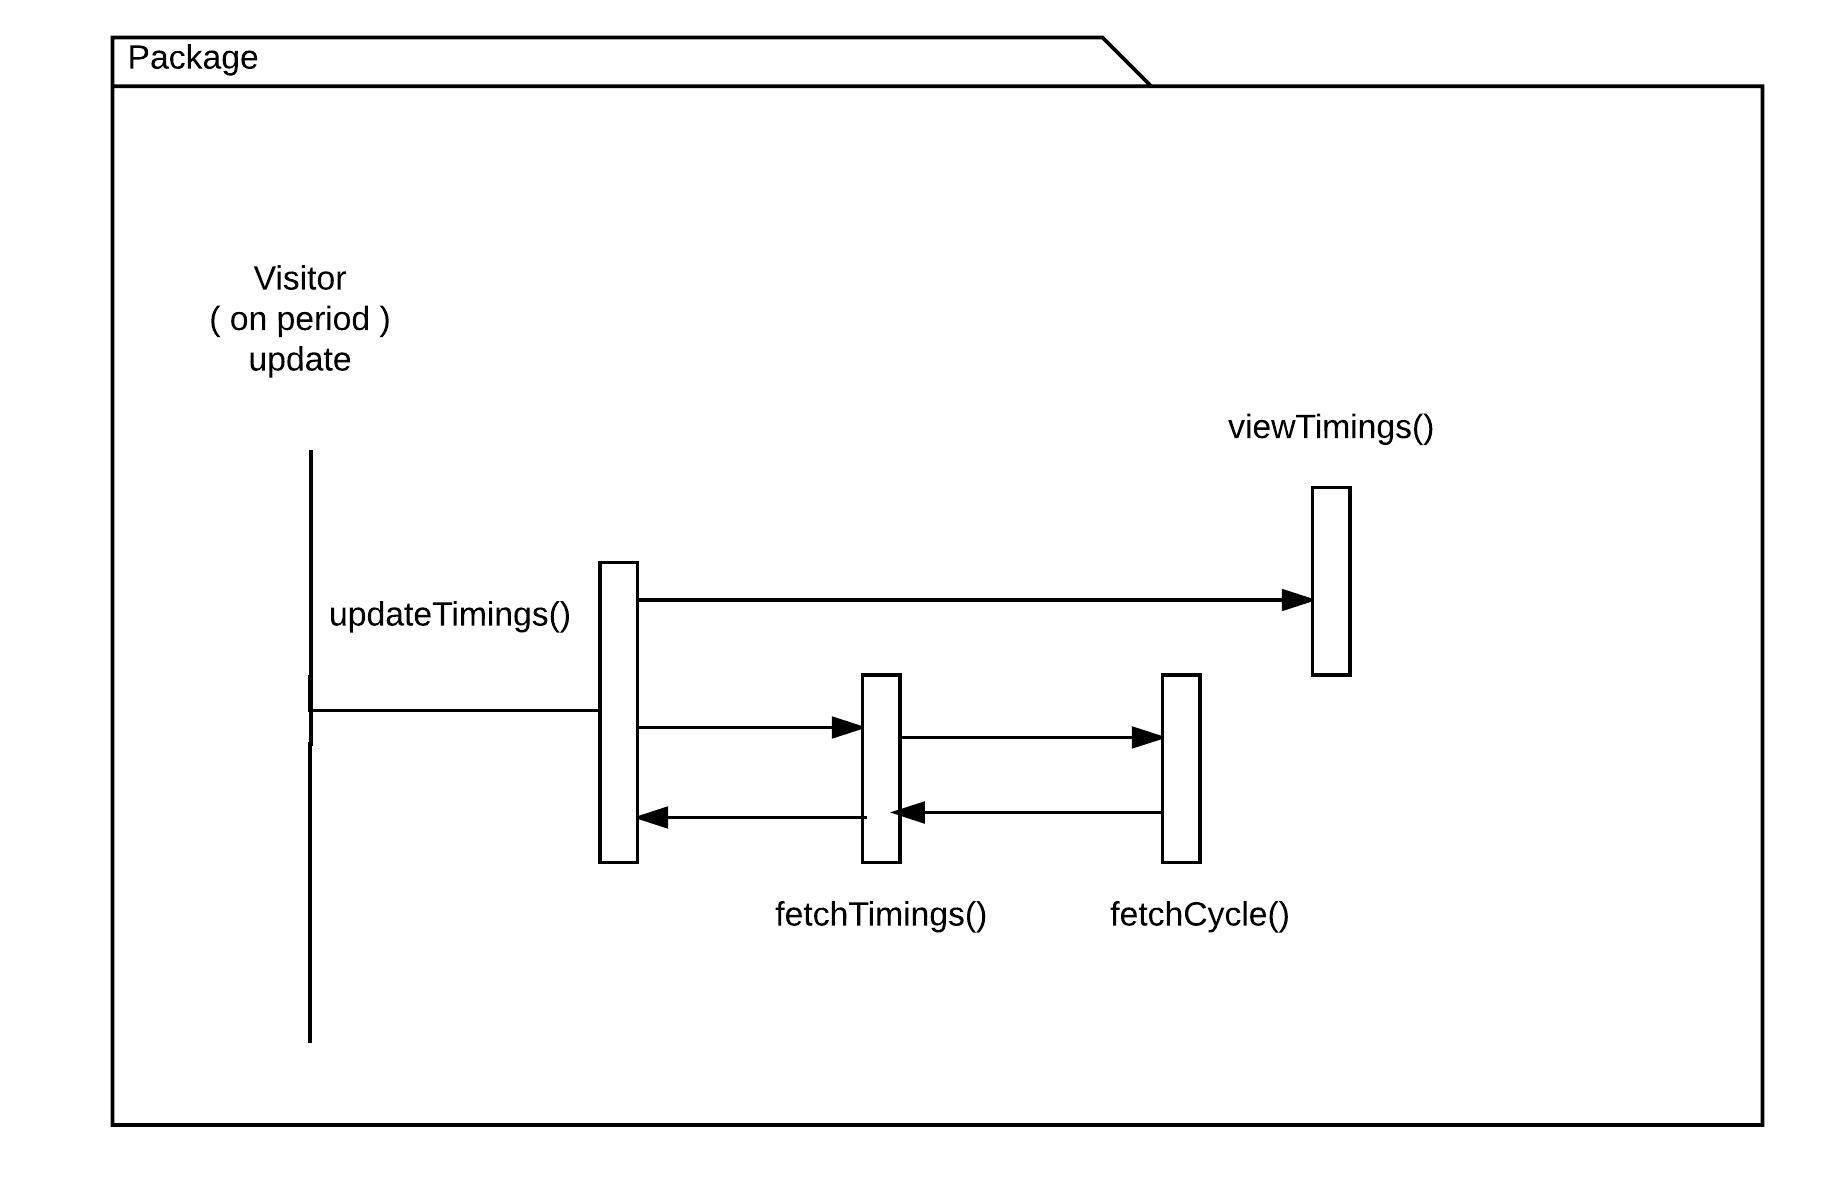
\includegraphics[scale=0.6]{Diagrams/Old Diagrams/User_Uncached_Sequence.jpeg}
		\end{center}
		\caption{Visitor's Usage Sequence (uncached data)}
	\end{figure}
	\begin{figure}[!h]
		\begin{center}
			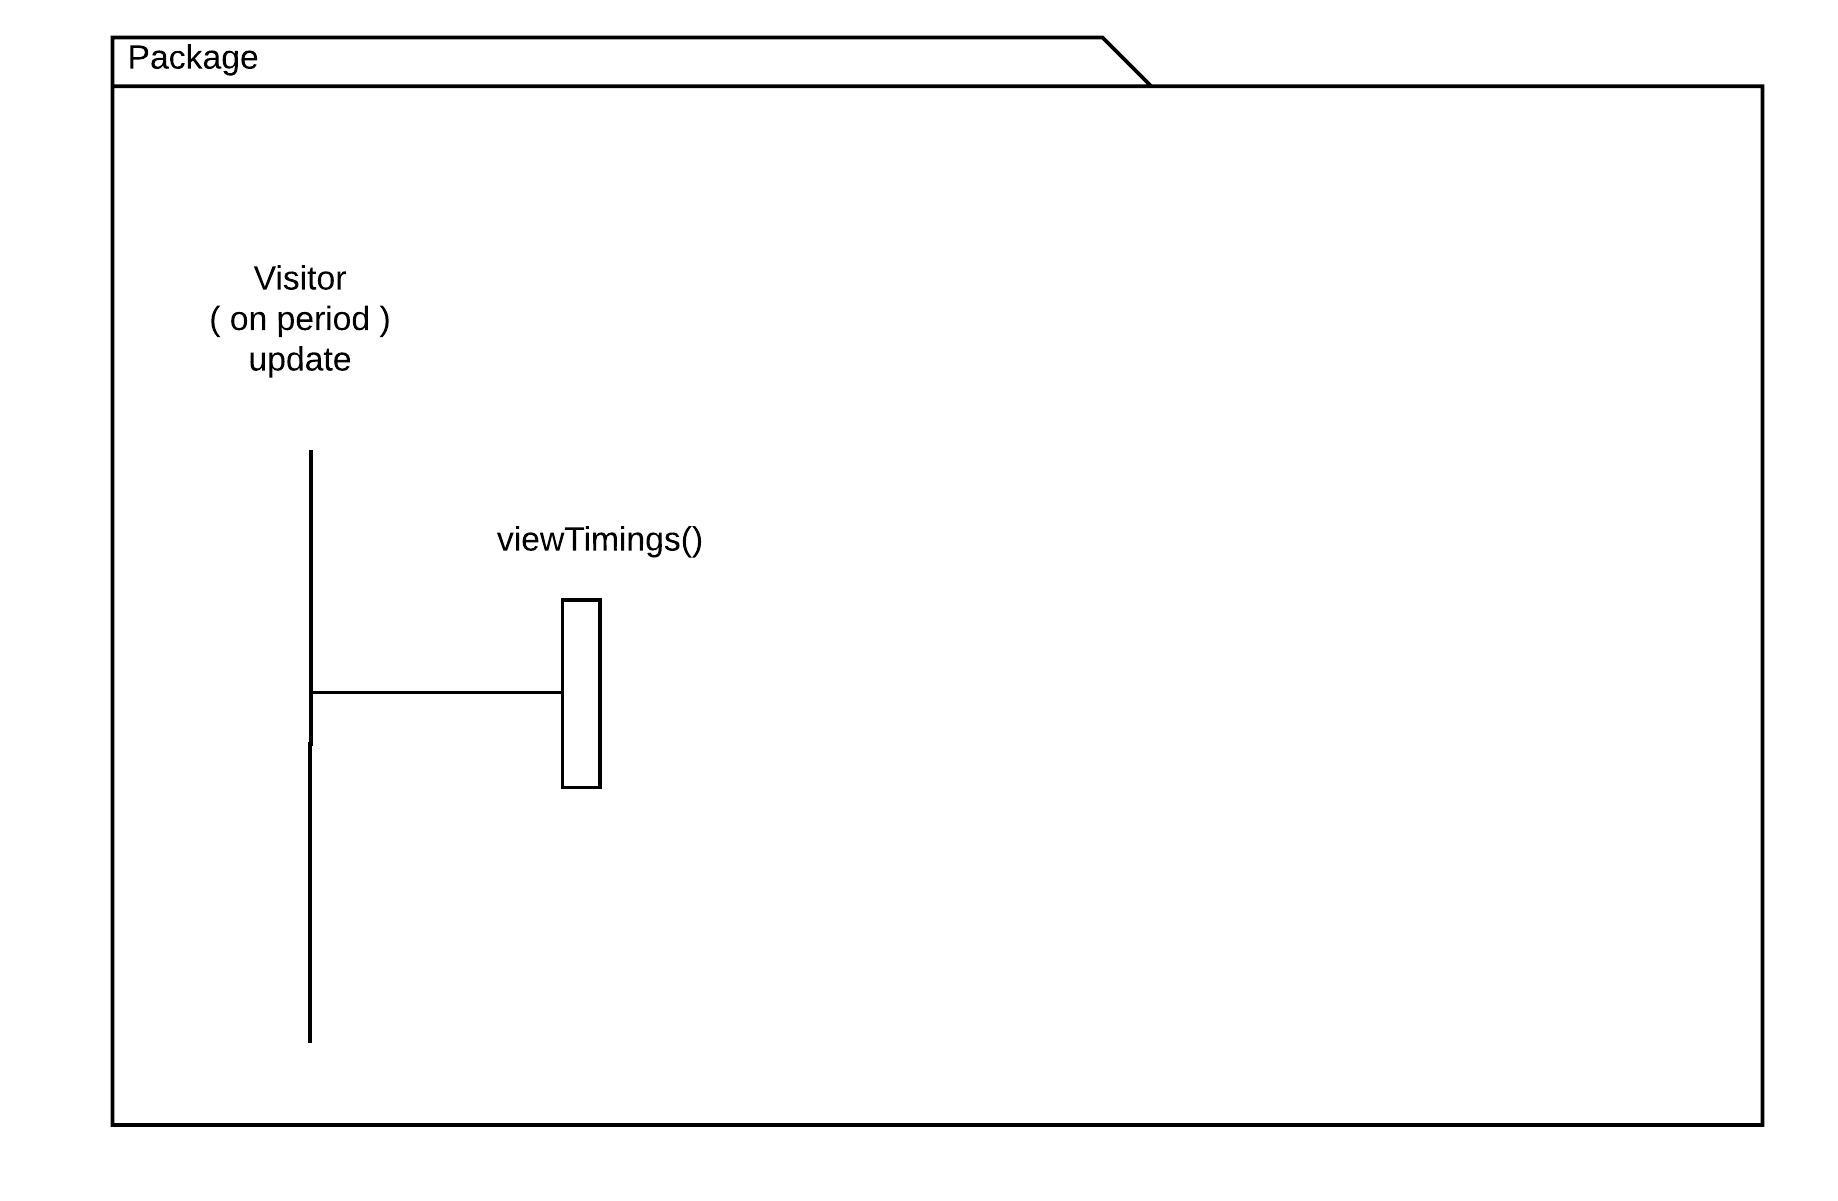
\includegraphics[scale=0.6]{Diagrams/Old Diagrams/User_Cached_Sequence.jpeg}
		\end{center}
		\caption{Visitor's Usage Sequence (cached data)}
	\end{figure}
\newpage
\subsubsection{Activity Diagram}
	\begin{figure}[!h]
		\begin{center}
			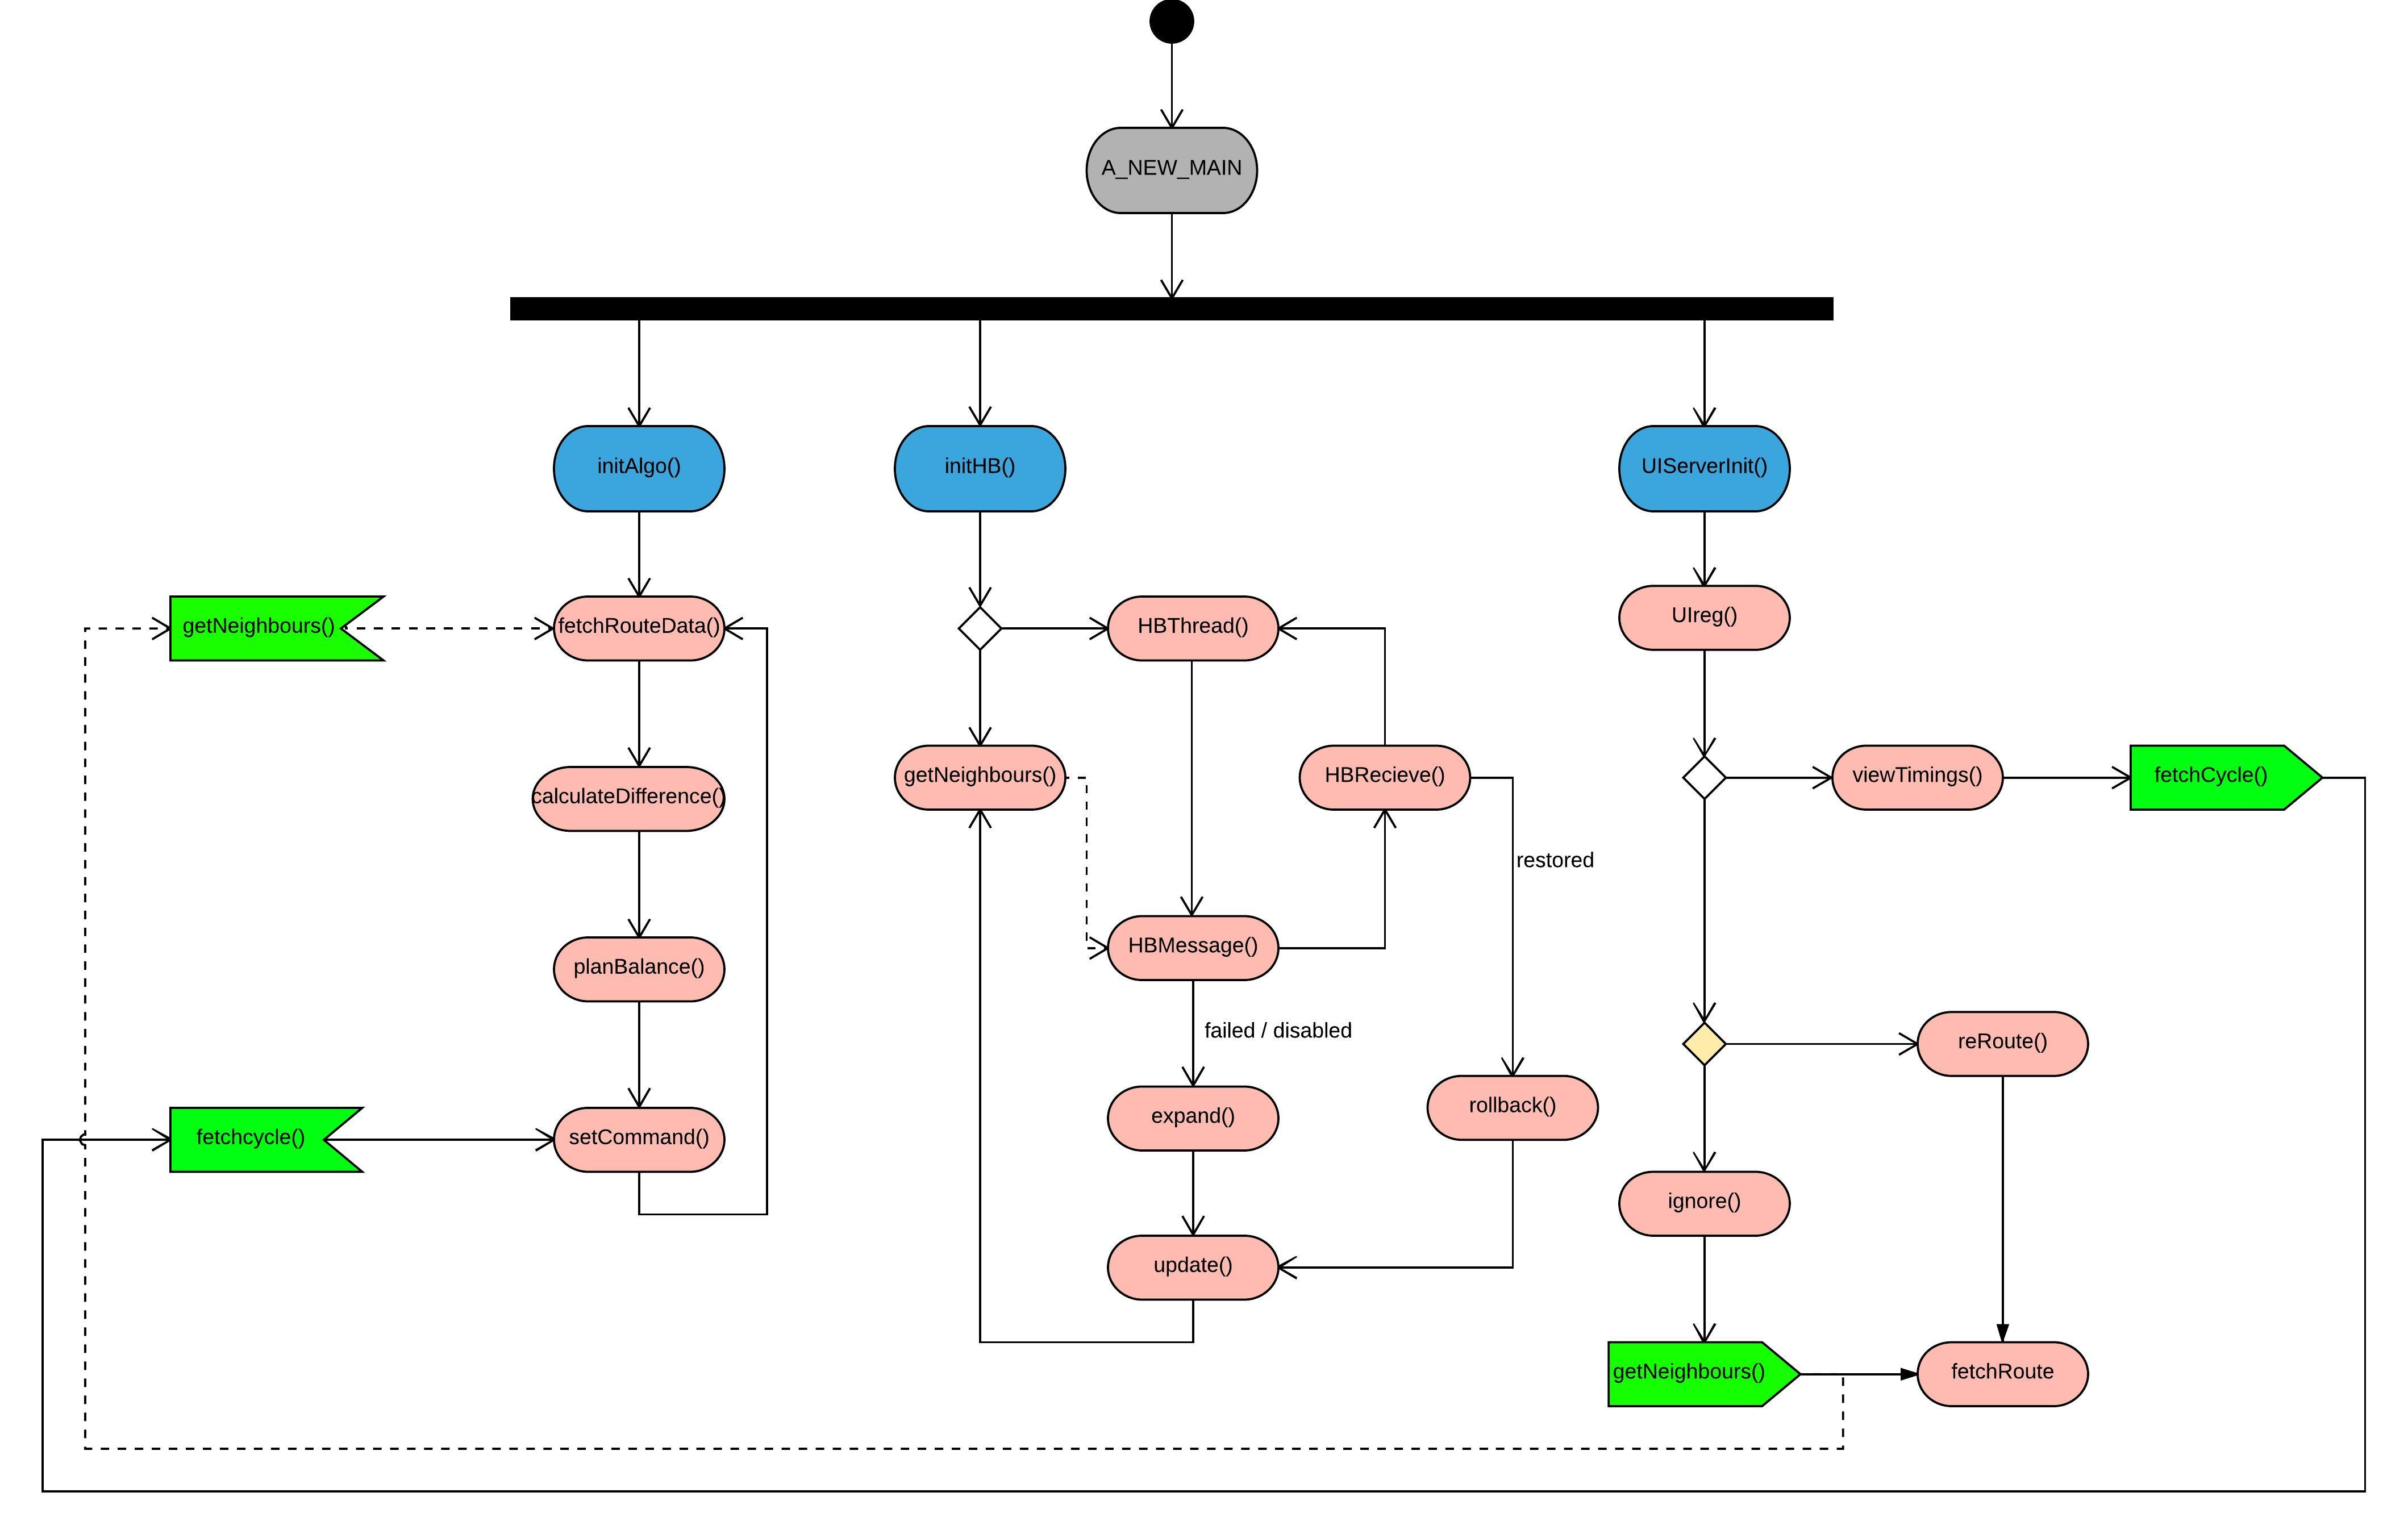
\includegraphics[scale=0.115]{Diagrams/Old Diagrams/Activity_Diagram.jpeg}
		\end{center}
		\caption{Activity Diagram}
	\end{figure}
\newpage

\subsection{Entity Relationship Diagram}
	\begin{figure}[!ht]
		\begin{center}
			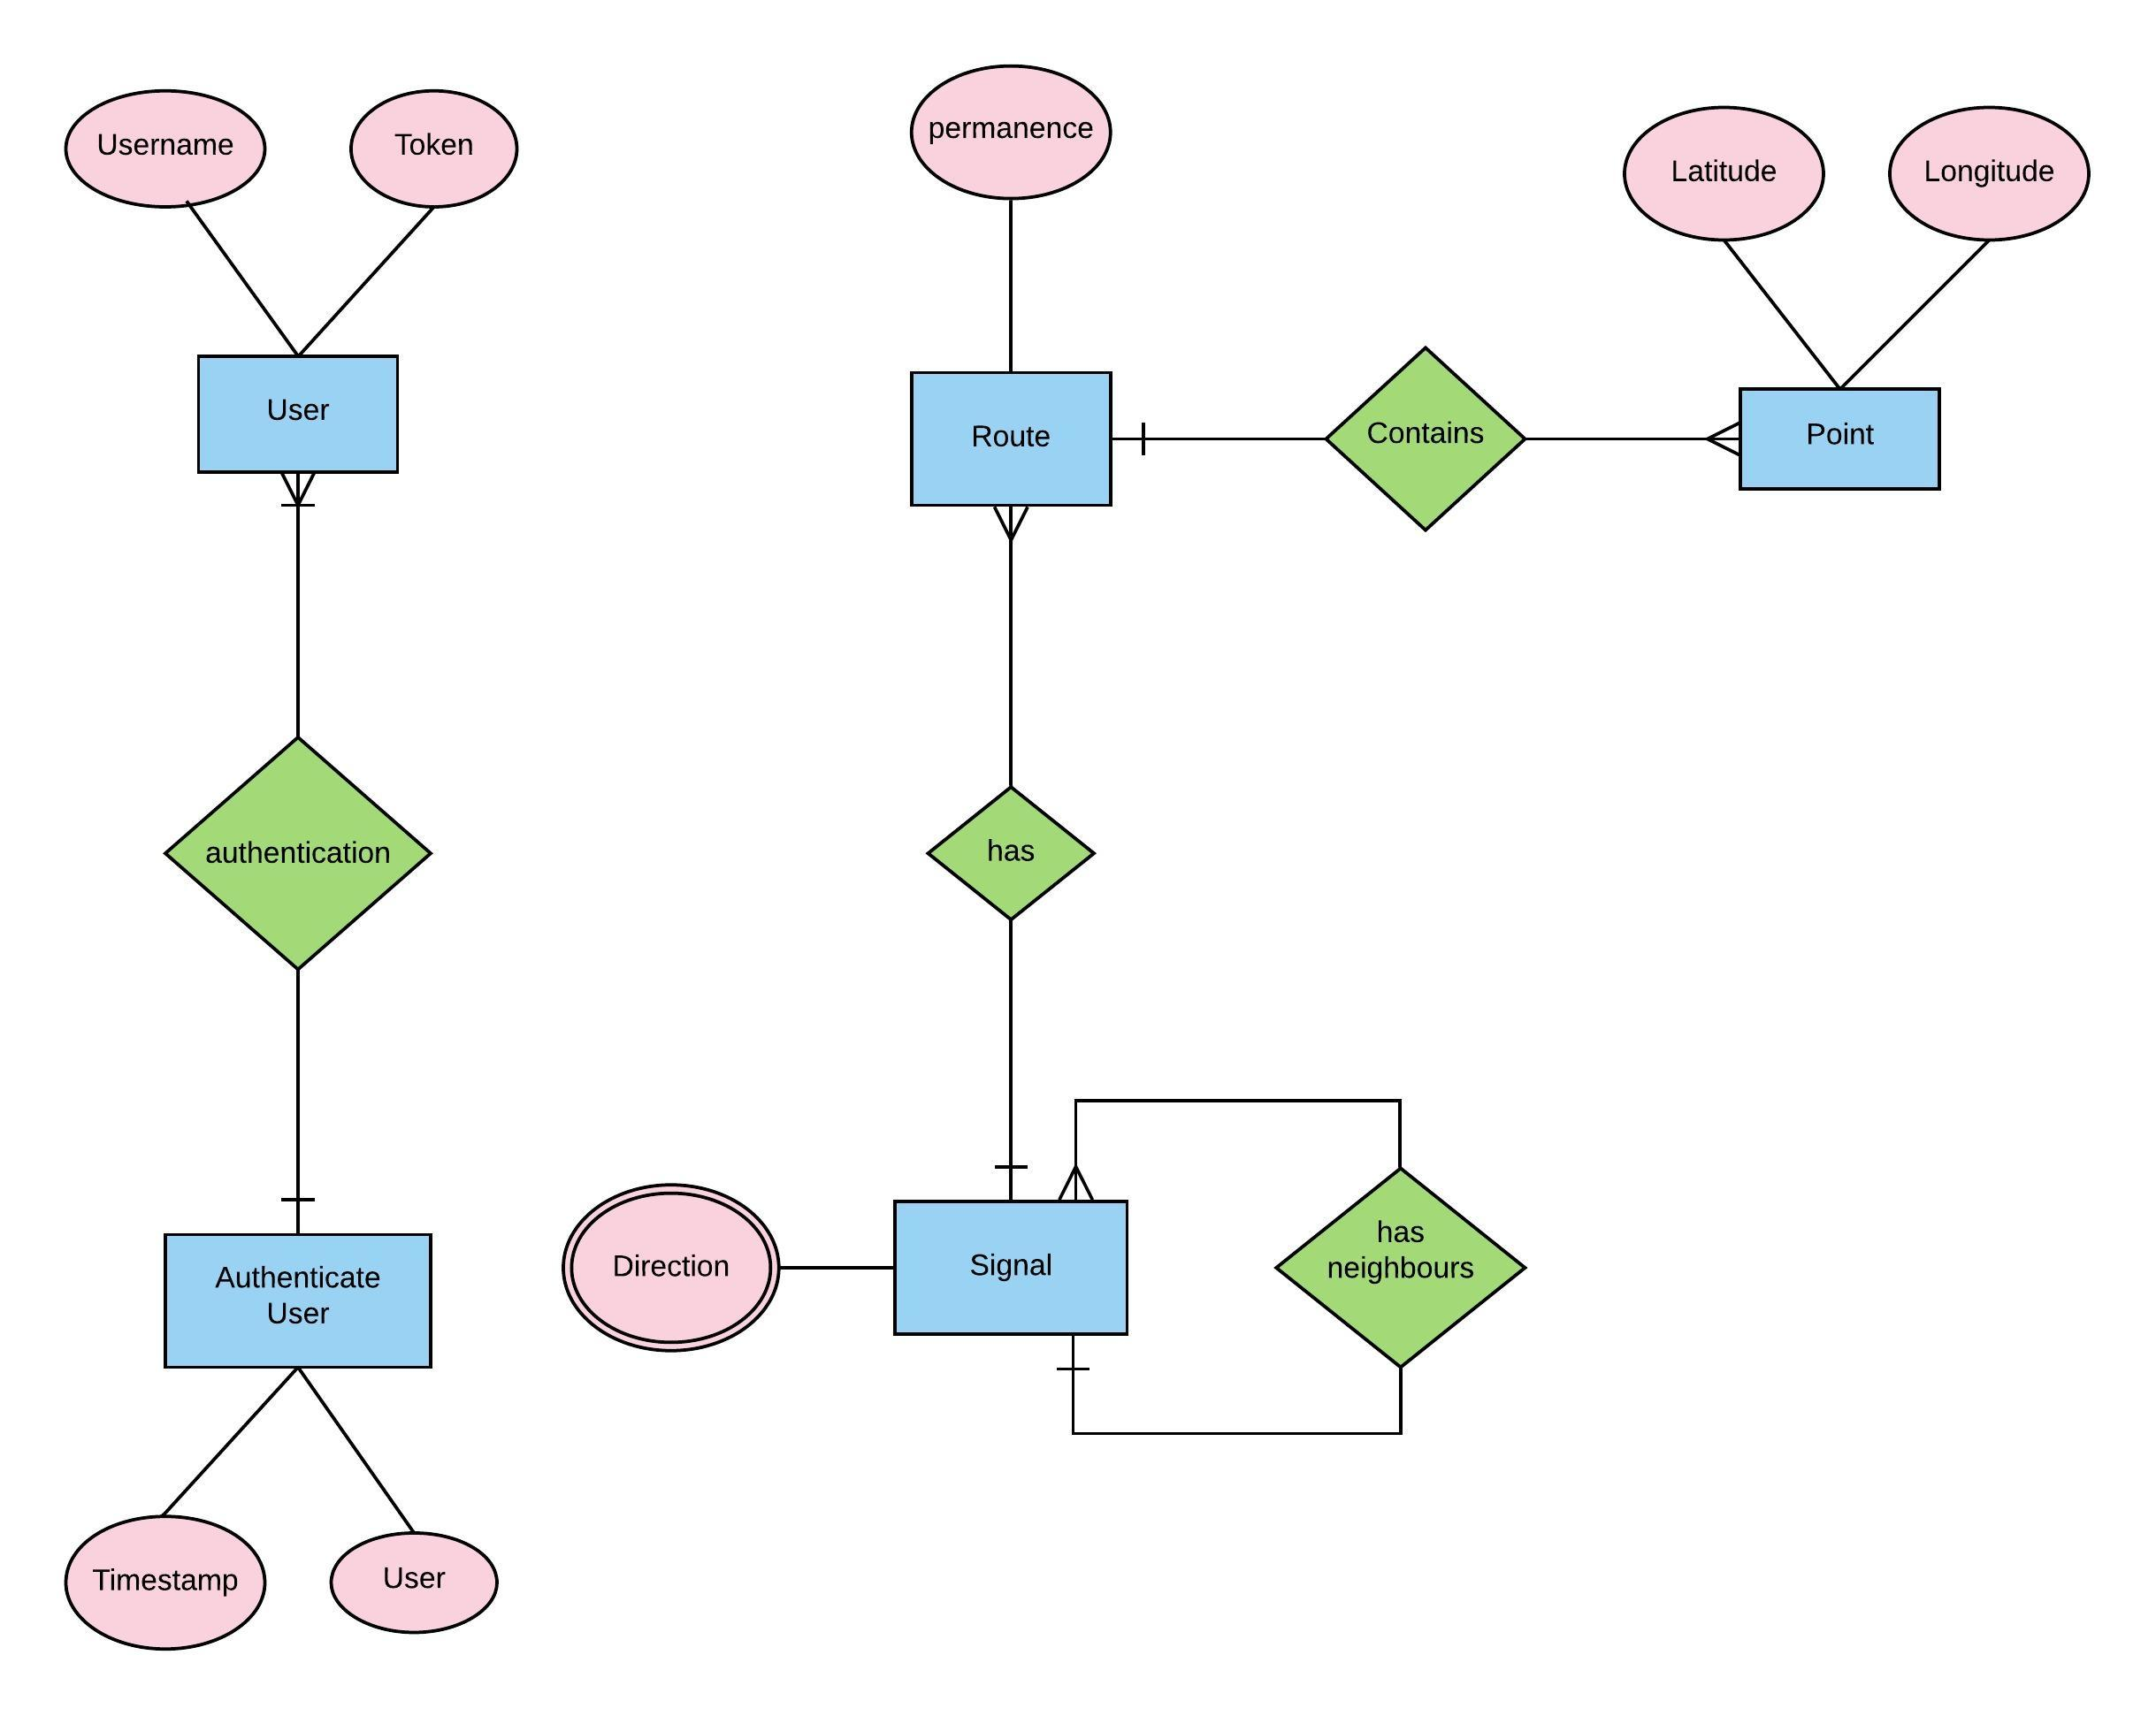
\includegraphics[scale=0.2]{Diagrams/Old Diagrams/ER_Diagram.jpeg}
		\end{center}
		\caption{ER Diagram}
	\end{figure}

\section{Planning Phase :}
\subsection{Software and Hardware Requirements:}
\begin{enumerate}
    \item 
    Software Requirements 
    \begin{itemize}
    		\item Linux Operating System (Arch, Debian) for Internet access to Google's Traffic API.
    		\item A representation of roads as Google's \emph{LatLong} Objects.
    		\item An interface to use/modify the Traffic Signal.
    \end{itemize}
    \item
    Hardware Requirements
    \begin{itemize}
    		\item Arduino UNO Rev.3 to control the signal.
    		\item A 3G or 4G enabled internet Dongle/WiFi NIC to use the Internet.
    \end{itemize}
    \item
    Front End Requirements:
    \begin{itemize}
    		\item JavaScript control to all Arduino Modules deployed in any route.
    		\item JavaScript access to GTAPI to view route's traffic conditions.
    \end{itemize}
    Back End Requirements:
    \begin{itemize}
    		\item JavaScript access to GTAPI to observe route section.
    		\item JavaScript access to Redis Database to access known LatLong Objects for route sections.
    \end{itemize}
\end{enumerate}
\subsection{Major milestones and deadlines:}
\begin{enumerate}
	\item
		Major Milestones:
		\begin{itemize}
			\item Validation of GTAPI usage and reliability.
			\item Developing Traffic Signal Controller in Python.
			\item Setting up Internet Access on Arduino. (Demo the GTAPI access).
			\item Developing the Traffic Management Algorithm.
			\item Testing and Tuning of above Algorithm using MOTUS Simulator.
			\item Using above Algorithm with Signal Controller.
		\end{itemize}
    \item
    Deadline for project completion: 18th March, 2018.
\end{enumerate}
\subsection{Structure of the database: }
\begin{enumerate}
    \item
	    JSON documents(A) storing (Latitude,Longitude) pairs for points on/along a route section; accessible using Route Section IDs.
   	\item
   		JSON documents(B) storing Route Section IDs and Controller IDs for each traffic signal; accessible using Controller IDs.
   	\item
   		JSON Documents(C) storing Direction:Controller IDs next to a given Controller ID for each traffic signal; accessible using Controller IDs.
   	\item
   		JSON Document(D) storing User's credentials (username and unique hashed token) for each User; accessible using username.
   	\item
   		JSON Document(E) storing Authenticated user with their Timestamp (time of login) for each logged-in user; accessible using username.
\end{enumerate}

\newpage

\section{Prototyping:}
The diagrams below are an early(demonstrational) model of the project's outcome.
	\begin{figure}[!h]
		\begin{center}
			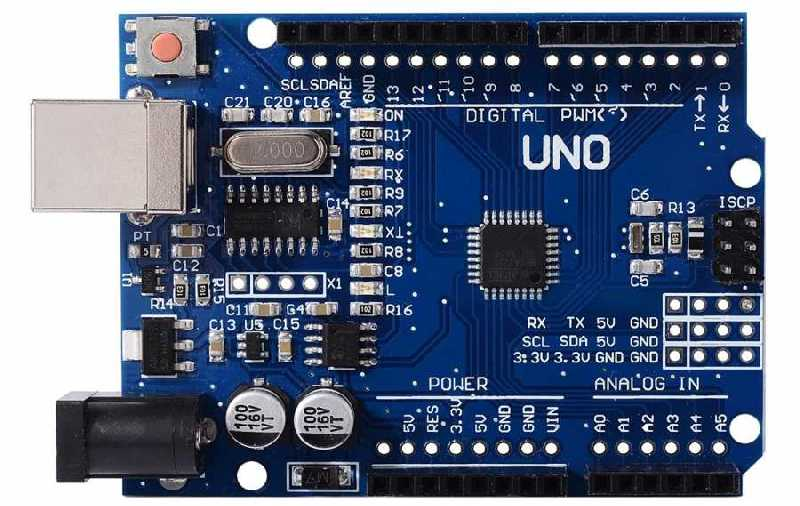
\includegraphics[scale=0.4]{UnoR3.jpg}
		\end{center}
		\caption{Hardware Prototype}
	\end{figure}
	\begin{figure}[!h]
		\begin{center}
			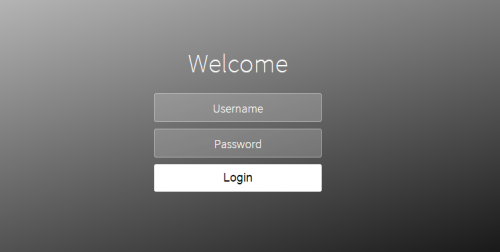
\includegraphics[scale=0.8]{Login.png}
		\end{center}
		\caption{Login UI}
	\end{figure}
	
	\newpage
	
	\begin{figure}[!h]
		\begin{center}
			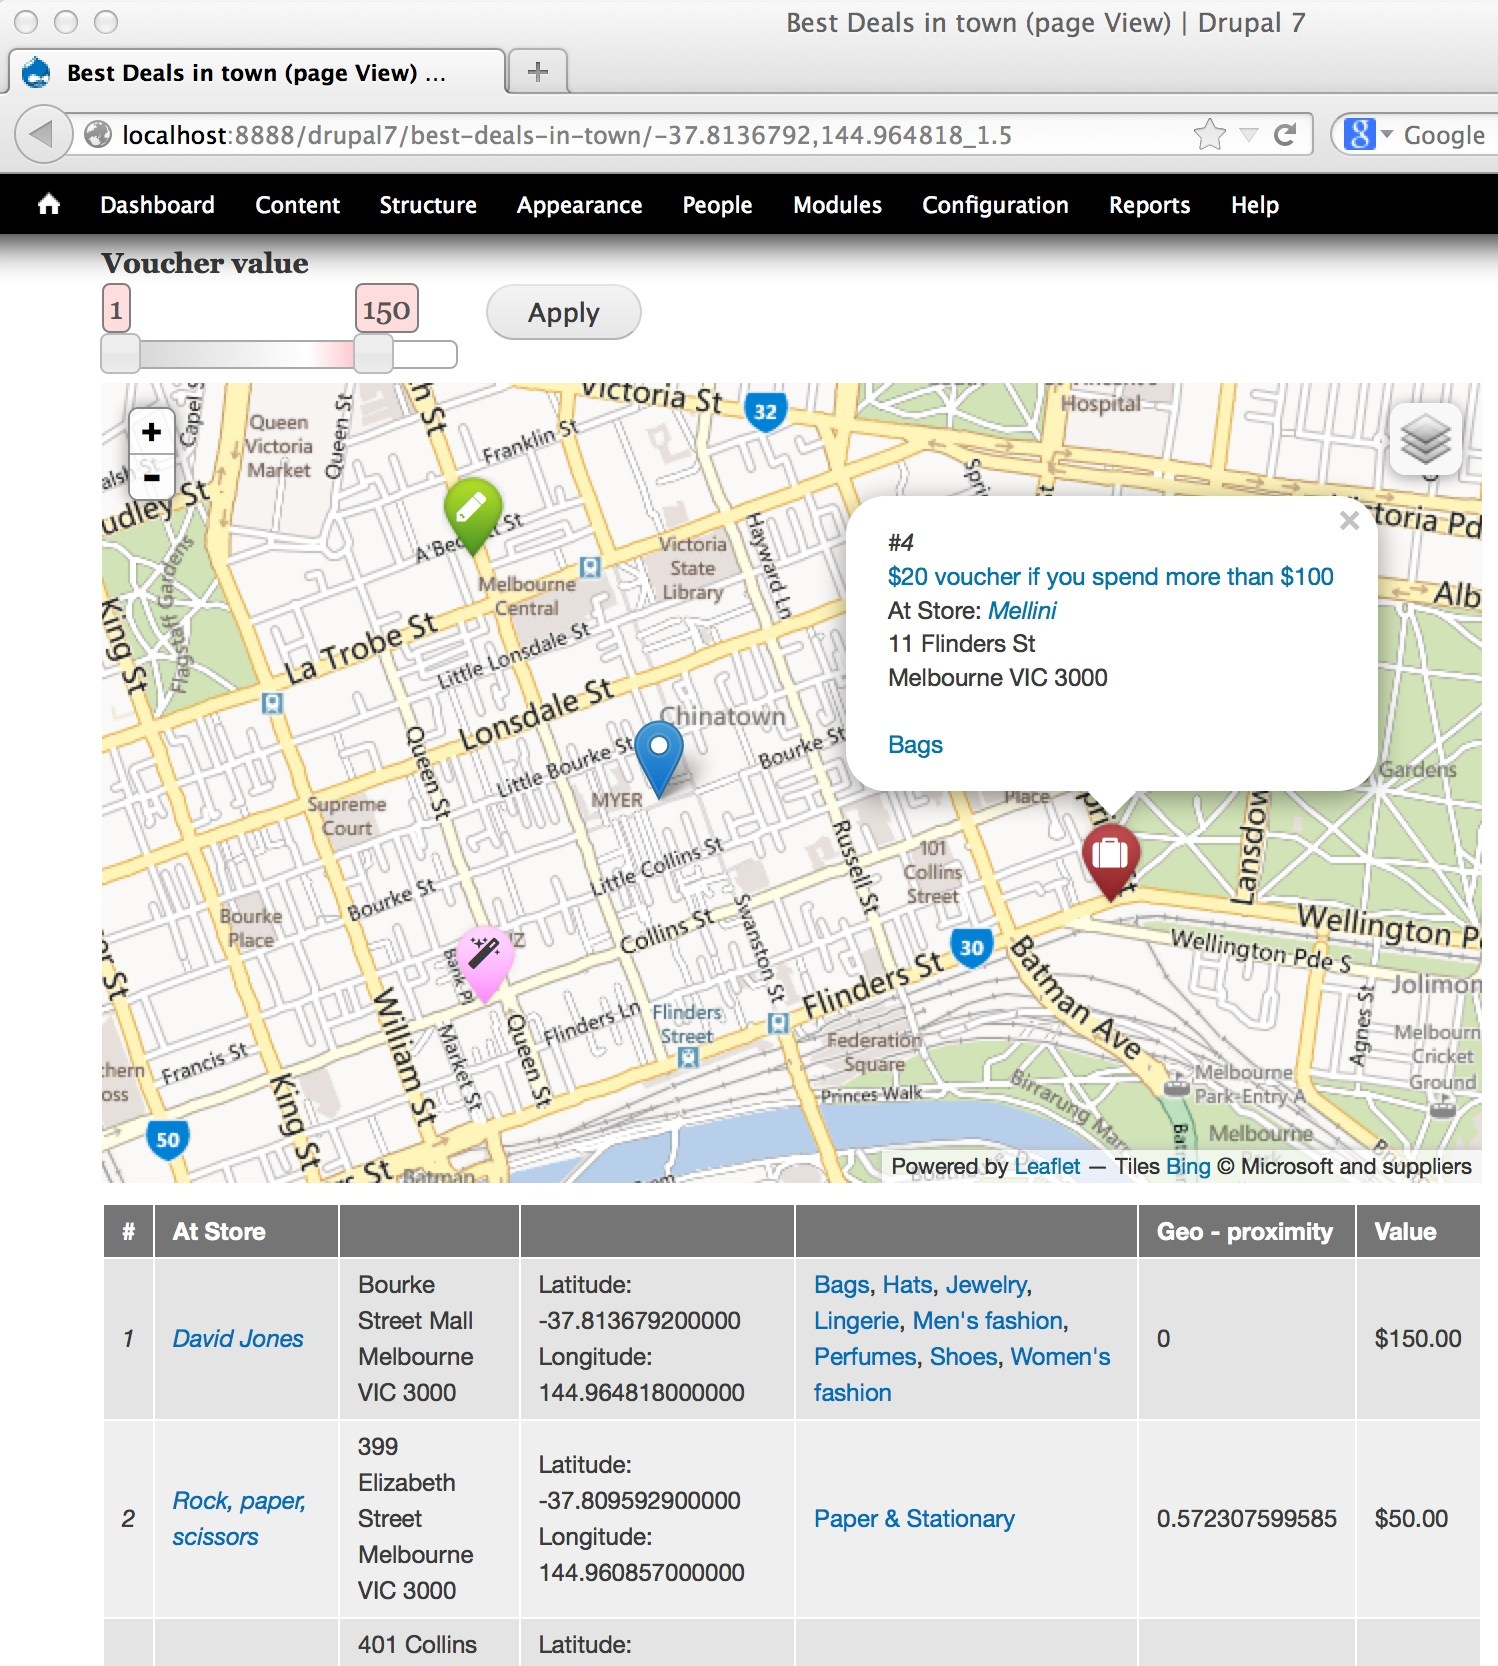
\includegraphics[scale=0.3]{Map.jpg}
		\end{center}
		\caption{Visitor UI}
	\end{figure}

All diagrams above are subject to changes in the future.

\newpage

\AddToShipoutPictureBG*{%
\begin{tikzpicture}[overlay,remember picture]
\draw[line width=1.5pt]
    ($ (current page.north west) + (0.7cm,-0.7cm) $)
    rectangle
    ($ (current page.south east) + (-0.7cm,0.7cm) $);
\draw[line width=1.5pt]
    ($ (current page.north west) + (0.9cm,-0.9cm) $)
    rectangle
    ($ (current page.south east) + (-0.9cm,0.9cm) $);
\end{tikzpicture}
}
\chapter{Conclusion}
\thispagestyle{empty}
\newpage
We have implemented a stable solution to a long standing Traffic problem. Our system is able to automatically handle traffic without any Human intervention. It actively looks for signs of Traffic Jam buildup and prevents it. The system achieves this in a decentralized manner such that there is no single point of control/failure. Comparing to leading technologies established in this field, our approach aims to reduce costs while providing the same level of efficiency. One can also note that our system is deployable anywhere without any major modifications required to the existing setup.
\newpage
\AddToShipoutPictureBG*{%
\begin{tikzpicture}[overlay,remember picture]
\draw[line width=1.5pt]
    ($ (current page.north west) + (0.7cm,-0.7cm) $)
    rectangle
    ($ (current page.south east) + (-0.7cm,0.7cm) $);
\draw[line width=1.5pt]
    ($ (current page.north west) + (0.9cm,-0.9cm) $)
    rectangle
    ($ (current page.south east) + (-0.9cm,0.9cm) $);
\end{tikzpicture}
}
\addcontentsline{toc}{chapter}{References}
\SkipTocEntry\chapter{References}
\thispagestyle{empty}
\newpage
\section*{References}
\begin{enumerate}[label={[\arabic*]}]
\item Alain Kibangou, et. al., “An Integrated and Scalable Platform for
 Proactive Event-Driven Traffic Management,” \textit{Arxiv.org}, 8th March 2017.

\item Carlos Gershenso, “Self-Organizing Traffic Lights,” \textit{Arxiv.org},
 5th Feb 2008.

\item Moshe E. Ben-Akiva, et. al., “A dynamic traffic assignment model
 for highly congested urban networks,” \textit{Elsevier}, 6th Feb 2012.

\item Pu Wang, et. al., “Understanding Road Usage Patterns in Urban
 Area,” \textit{SCIENTIFIC REPORTS}, vol 2, no. 1001, 20 December 2012.

\item Nasrin Taherkhani and Samuel Pierre, “Centralized and Localized
 Data Congestion Control Strategy for Vehicular Ad Hoc Networks Using
 a Machine Learning Clustering Algorithm,” \textit{IEEE TRANSACTIONS ON
 INTELLIGENT TRANSPORTATION SYSTEMS}, March 20, 2016.

\end{enumerate}
\newpage

\AddToShipoutPictureBG*{%
\begin{tikzpicture}[overlay,remember picture]
\draw[line width=1.5pt]
    ($ (current page.north west) + (0.7cm,-0.7cm) $)
    rectangle
    ($ (current page.south east) + (-0.7cm,0.7cm) $);
\draw[line width=1.5pt]
    ($ (current page.north west) + (0.9cm,-0.9cm) $)
    rectangle
    ($ (current page.south east) + (-0.9cm,0.9cm) $);
\end{tikzpicture}
}

\addcontentsline{toc}{chapter}{Annexure - A}
\SkipTocEntry\chapter{Annexure - A}
\thispagestyle{empty}
\newpage
\section*{Table 2 - IDEA Matrix}
\addcontentsline{lot}{table}{5.1 \hspace*{10pt}IDEA Matrix}
\begin{figure}[!h]
	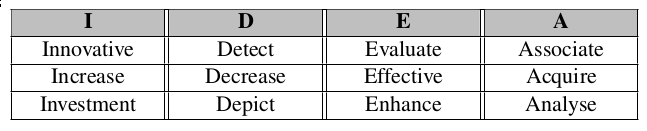
\includegraphics[scale=0.75]{IDEA_Matrix.png}
\end{figure}

\vspace*{2cm}

\begin{table}[!h]
	\centering
	\begin{Large}
	\begin{tabular}{| c | p{9cm} |}
		\toprule
		 Innovate & Traffic systems are either centralized or uncoordinated or need a lot of additions to the installation site. Here, the system uses only one addition which can be a replacement to existing signal control hardware and is decentralized which is \textbf{innovative}.\\
		Increase & As the system uses real-time data from GTAPI (which is cached), the efficiency of the system will \textbf{increase}.\\
		Investment & As the system uses commodity hardware, \textbf{investment is minimal} and installation is easy.\\
		\bottomrule
	\end{tabular}
	\end{Large}
\end{table}

\newpage \vspace*{2cm}

\begin{table}[!h]
	\centering
	\begin{Large}
	\begin{tabular}{| c | p{9cm} |}
		\toprule
		Detect & The system will \textbf{detect} the signs of traffic buildup and makes changes to the signal timings dynamically.\\
		Decrease & The algorithm will \textbf{decrease} the buildup by increasing green time along the route and increasing overall cycle timings for heavily loaded signals.\\
		Depict & The system UI \textbf{depicts} the timings and status of each traffic signal in real-time.\\
		\bottomrule
	\end{tabular}
	\end{Large}
\end{table}

\vspace*{2cm}

\begin{table}[!h]
	\centering
	\begin{Large}
	\begin{tabular}{| c | p{9cm} |}
		\hline
		Evaluate & The algorithm \textbf{evaluates} the densities of traffic in each lane to decide timings\\
		Effective & The densities are obtained in real-time allowing for steady and tiny changes in timings to be highly \textbf{effective}.\\
		Enhance & The system can be \textbf{enchanced} by improving decisions about changes and their amount.\\
		\hline
	\end{tabular}
	\end{Large}
\end{table}

\newpage \vspace*{5cm}

\begin{table}[!h]
	\centering
	\begin{Large}
	\begin{tabular}{| c | p{9cm} |}
		\hline
		Associate & The project \textbf{associates} incremental approach to large distributed networks to allow optimal solutions to emerge.\\
		Acquire & The density data of each lane is \textbf{acquired} from GTAPI.\\
		Analyse & The system \textbf{analyzes} current density information and previous cycle's densities to produce current timings.\\
		\hline
	\end{tabular}
	\end{Large}
\end{table}

\newpage

\AddToShipoutPictureBG*{%
\begin{tikzpicture}[overlay,remember picture]
\draw[line width=1.5pt]
    ($ (current page.north west) + (0.7cm,-0.7cm) $)
    rectangle
    ($ (current page.south east) + (-0.7cm,0.7cm) $);
\draw[line width=1.5pt]
    ($ (current page.north west) + (0.9cm,-0.9cm) $)
    rectangle
    ($ (current page.south east) + (-0.9cm,0.9cm) $);
\end{tikzpicture}
}
\addcontentsline{toc}{chapter}{Annexure - B}
\SkipTocEntry\chapter{Annexure - B}
\thispagestyle{empty}
\newpage \vspace*{3.5cm}

\section*{Table 3 - Test Cases}
\addcontentsline{lot}{table}{6.1 \hspace*{10pt}Test Cases}
\begin{table}[!ht]
	\centering
	\begin{tabular}{| p{1cm} | p{7cm} | p{4cm} | p{4cm} |}
		\toprule
		\textbf{Test ID} & \textbf{Test Case Description} & \textbf{Input} & \textbf{Expected Output} \\
		\midrule
%		& & & \\
		1 & User enters a Correct Username \& Correct Password & Valid Username \& Valid Password & Access Granted \\
		\hline
		2 & User enters an Incorrect Username \& Correct Password & Invalid Username \& Valid Password & Access Denied \\
		\hline
		3 & User enters a Correct Username \& Incorrect Password & Valid Username \& Invalid Password & Access Denied \\
		\hline
		4 & User enters an Incorrect Username \& Incorrect Password & Invalid Username \& Invalid Password & Access Denied \\
		\hline
		5 & User wants to modify routes & Valid changes & Changes saved in UI Buffer\\
		\hline
		6 & User wants to modify routes & Invalid changes & Changes saved in UI Buffer \\
		\hline
		7 & User wants to save modified routes & Valid changes & Changes saved in Redis Database \\
		\hline
		8 & User wants to save modified routes & Invalid Changes & Changes not saved \& are discarded \\
		\hline
		& & & \\
		9 & User wants to modify Node status & Switch ON & Node switched ON \\
		\hline
		& & & \\
		10 & User wants to modify Node status & Switch OFF & Node switched OFF \\
		\hline
		& & & \\
		11 & User wants to modify Node status & Switch ON then OFF & No Change in Node status \\
		\hline
		12 & User wants to modify Node status & Switch OFF then ON & No Change in Node status \\
		\hline
		13 & User wants to modify Node status & Combination of 0/1 cases of type 11 and m cases of 12 & Output of case type 11 \\
		\bottomrule
	\end{tabular}
\end{table}

\newpage

\AddToShipoutPictureBG*{%
\begin{tikzpicture}[overlay,remember picture]
\draw[line width=1.5pt]
    ($ (current page.north west) + (0.7cm,-0.7cm) $)
    rectangle
    ($ (current page.south east) + (-0.7cm,0.7cm) $);
\draw[line width=1.5pt]
    ($ (current page.north west) + (0.9cm,-0.9cm) $)
    rectangle
    ($ (current page.south east) + (-0.9cm,0.9cm) $);
\end{tikzpicture}
}
\addcontentsline{toc}{chapter}{Annexure - C}
\SkipTocEntry\chapter{Annexure - C}
\thispagestyle{empty}
\newpage
\vspace*{2cm}
\section*{Table 4 - Progress Report}
\addcontentsline{lot}{table}{7.1 \hspace*{10pt}Progress Report}
\begin{table}[!ht]
	\centering
	\begin{tabular}{| p{0.7cm} | p{2.8cm} | p{7cm} | c |}
		\toprule
		Sr. No. & Day and Date & Topics Discussed & Suggestion of Project Guide \\
		\midrule
		1 & Tuesday, $22^{nd}$ August 2017 & Base Paper, Topic, Tools Decided. & \\
		2 & Monday, $18^{th}$ September 2017 & Seeking Algorithm class/style. & \\
		3 & Thursday, $28^{th}$ September 2017 & Partial Presentation made. & \\
		4 & Wednesday, $11^{th}$ October 2017 & Synopsis made. & \\
		5 & Tuesday, $24^{th}$ November 2017 & Partial UML Diagrams completed (Structural). & \\
		6 & Monday, $11^{th}$ December 2017 & SRS Textual Content completed Partial Behavioural Diagrams completed (Use case, Statechart, Sequence). & \\
		7 & Wednesday, $13^{th}$ December 2017 & Completed UML Diagrams (Activity) and ER Diagram. Partial Project Report completed. & \\
        8 & February 2018 End & Data Collection Completed & \\
        9 & Mid January 2018 & Algorithm Design Completed & \\
        10 & January 2018 End & Hardware Design and Testing Completed & \\
        11 & February 2018 End & UI Design and Testing Completed & \\
        12 & Mid March 2018 & Algorithm Testing using Data Collected & \\
		\bottomrule
	\end{tabular}
\end{table}
\end{document}
